\documentclass[11pt]{article}
\usepackage[T1]{fontenc}
\usepackage[utf8]{inputenc}
\usepackage{lmodern}
\usepackage{mathpazo}
\usepackage{amsmath,amssymb,amsthm,mathtools}
\usepackage[margin=1.02in]{geometry}
\usepackage{microtype}
\usepackage{enumitem,booktabs,longtable,array}
\usepackage{xcolor,xurl,listings}
\usepackage{tikz}
\usepackage[colorlinks=true,linkcolor=blue!45!black,citecolor=blue!45!black,urlcolor=blue!45!black]{hyperref}
\hypersetup{pdftitle={The exact reconstruction threshold for the three-state symmetric channel},pdfauthor={OpenAI}}
\newtheorem{theorem}{Theorem}[section]
\newtheorem{lemma}[theorem]{Lemma}
\newtheorem{proposition}[theorem]{Proposition}
\newtheorem{corollary}[theorem]{Corollary}
\theoremstyle{definition}
\newtheorem{definition}[theorem]{Definition}
\theoremstyle{remark}
\newtheorem{remark}[theorem]{Remark}
\newcommand{\E}{\mathbb E}
\newcommand{\PP}{\mathbb P}
\newcommand{\av}[1]{\langle #1\rangle}
\newcommand{\R}{\mathbb R}
\setlist{topsep=4pt,itemsep=3pt,parsep=0pt}
\setlength{\emergencystretch}{2em}
\numberwithin{equation}{section}
\lstset{basicstyle=\ttfamily\scriptsize,columns=fullflexible,keepspaces=true,
  breaklines=true,breakatwhitespace=false,showstringspaces=false,
  numbers=left,numberstyle=\tiny\color{gray},numbersep=7pt,
  xleftmargin=1.5em,frame=single,rulecolor=\color{black!25},
  framerule=.3pt,aboveskip=8pt,belowskip=8pt,tabsize=4}
\pdfminorversion=5
\ifdefined\pdfinfoomitdate\pdfinfoomitdate=1\fi
\ifdefined\pdftrailerid\pdftrailerid{}\fi

\title{The exact reconstruction threshold\\for the three-state symmetric channel}
\author{OpenAI}
\date{September 25, 2026}
\begin{document}
\maketitle
\begin{abstract}
We determine the exact reconstruction threshold for the symmetric
three-state broadcast process on every regular $b$-ary tree, $b\ge2$,
and every observed Poisson Galton--Watson tree of mean $d>1$.
Reconstruction occurs exactly when $d\lambda^2>1$, with $d=b$ in the
regular model; there is non-reconstruction at equality for either sign
of the channel parameter. The Poisson advantage is averaged over trees
and spins without conditioning on survival. This resolves the all-degree
three-state regular-tree prediction.
Combining the Poisson theorem with known tree-to-graph and algorithmic
results gives the exact weak-recovery threshold for the symmetric
three-community sparse stochastic block model with independent uniform
labels, fixed within- and between-community rates $a,b>0$, and mean
degree $(a+2b)/3>1$: recovery is possible exactly when
$(a-b)^2>3(a+2b)$. Above this threshold it is achievable in
$O(n\log n)$ time; at or below it, weak recovery is
information-theoretically impossible.
\end{abstract}
\tableofcontents
\section{Introduction}\label{sec:introduction}
The reconstruction problem asks whether many distant, noisy descendants
retain information about their common ancestor. On a tree, the growth in
the number of descendants competes with the loss of information across
each edge. For a symmetric channel with nontrivial eigenvalue $\lambda$
and mean offspring number $d$, the Kesten--Stigum condition
$d\lambda^2>1$ gives reconstruction. Whether this condition is also
necessary depends on the channel. We determine the answer for three
states at every branching parameter in two basic tree families.
Through existing tree-to-graph and algorithmic results, the Poisson
theorem also determines the weak-recovery threshold for the symmetric
three-community sparse stochastic block model with positive connectivity
parameters and mean degree greater than one.

\subsection{Model and result}
Let the root spin $\sigma_\rho$ be uniform on $\{1,2,3\}$. Along each
edge, independently conditional on its parent spin, transmit through
\begin{equation}\label{eq:channel}
 K_\lambda(i,j)=
 \begin{cases}
 (1+2\lambda)/3,&i=j,\\
 (1-\lambda)/3,&i\ne j,
 \end{cases}
 \qquad -\tfrac12\le\lambda\le1.
\end{equation}
The tree is either the rooted $b$-ary tree, with an integer $b\ge2$
children at every vertex, or a Galton--Watson tree with independent
$\operatorname{Pois}(d)$ offspring counts, where $d>1$.
For the regular model set $d=b$. The tree is independent of the root
spin. The observation at depth $\ell$ consists of the unlabelled tree
$T_{\le\ell}$ through that depth together with the spins attached to its
vertices $\partial T_\ell$ at depth $\ell$; neither interior spins nor
an ordering of siblings are observed. Define
\begin{equation}\label{eq:advantage}
 a_\ell=\E\left\|
 \PP(\sigma_\rho=\cdot\mid T_{\le\ell},\sigma_{\partial T_\ell})
 -\operatorname{Unif}\{1,2,3\}\right\|_{\mathrm{TV}}.
\end{equation}
In the Poisson case this expectation includes both the tree and the
spins, \emph{without conditioning on survival}. Reconstruction means
$\lim_{\ell\to\infty}a_\ell>0$; non-reconstruction means that this
limit is zero. The limit exists by information degradation.

\begin{theorem}[Exact threshold]\label{thm:threshold}
For every integer $b\ge2$ in the regular model and every real $d>1$
in the Poisson model, reconstruction occurs if and only if
\[
 d\lambda^2>1,
\]
with $d=b$ in the regular case. At every admissible equality
$d\lambda^2=1$, there is non-reconstruction.
\end{theorem}
Thus the positive threshold is $\lambda=d^{-1/2}$. On the negative
side reconstruction occurs precisely when $d>4$ and
$-1/2\le\lambda<-d^{-1/2}$. In particular, the three-coloring channel
$\lambda=-1/2$ is non-reconstructible at branching parameter four in
both models.

\subsection{History and significance}
The branching-process work of Kesten and Stigum~\cite{KestenStigum1966}
underlies the classical second-moment reconstruction bound. Broadcasting
and its relation to the Ising model were developed by Evans, Kenyon,
Peres, and Schulman~\cite{EvansEtAl2000}. For more than two states,
nonlinear information in the boundary can change the threshold. This
possibility occurs for symmetric channels with five or more states
\cite[Theorem~1.2]{Sly2011}; the three-state assertion therefore needs
more than the second-moment bound.

M\'ezard and Montanari~\cite[Conjecture~2 and the following paragraph]{MezardMontanari2006}
predicted sharpness of the Kesten--Stigum bound for three-state symmetric
channels of either sign up to a branching cutoff, and proposed the
extension to all branching parameters. See also Conjecture~1 of
Sly~\cite{Sly2011} for the all-degree regular-tree formulation.
Sly proved this for all sufficiently large regular branching parameters,
including non-reconstruction at equality
\cite[Theorem~1.1]{Sly2011}. Mossel, Sly, and Sohn established the
corresponding large-mean Poisson-tree result, for both signs and including
equality \cite[Theorem~1.12]{MosselSlySohn2025}.
At small degrees, Bhatnagar and Maneva developed finite representations
of posterior laws and proved, among other bounds, non-reconstruction
for three-colorings on the regular ternary tree
\cite[Theorem~12]{BhatnagarManeva2011}.
Theorem~\ref{thm:threshold} removes the large-branching restriction in
these two tree families. It resolves the three-state regular-tree
prediction in its all-degree form and includes the low-branching and
coloring endpoints for the observed Poisson tree.

For the symmetric stochastic block model, the cavity-method analysis of
Decelle, Krzakala, Moore, and Zdeborov\'a predicted the Kesten--Stigum
transition in the assortative three-community case
\cite[Section~IV.A]{DecelleEtAl2011}.
Ricci-Tersenghi, Semerjian, and Zdeborov\'a gave further evidence for the
three-state prediction for either sign, through local analysis of the
posterior recursion and numerical cavity solutions
\cite[Sections~III.D.1 and~IV.H]{RicciTersenghiEtAl2019}.
Mossel, Sly, and Sohn proved information-theoretic impossibility at and
below the Kesten--Stigum bound for three or four communities when the
mean degree is sufficiently large
\cite[Theorem~1.5]{MosselSlySohn2025}.
Their tree-to-graph transfer has no large-degree restriction
\cite[Theorem~2.1]{MosselSlySohn2025}.
Together with the above-threshold algorithm of Abbe and Sandon
\cite[Corollary~1 and Lemma~1]{AbbeSandon2018}, the Poisson part of our
theorem therefore gives the exact three-community weak-recovery threshold
stated in Corollary~\ref{cor:sbm} below.

A related three-state model with branch-dependent couplings on a binary
Cayley tree is studied by Mukhamedov and Ak{\i}n~\cite{MukhamedovAkin2026}.
Their work concerns disordered translation-invariant Gibbs measures and
their extremality; our theorem concerns the same homogeneous symmetric
channel on every edge of the regular or observed Poisson tree.

\subsection{Proof strategy and its precedents}
For a root posterior $p=(p_1,p_2,p_3)$, write $m_i=3p_i$ and identify
the three spin labels with $1,\omega,\omega^2$, where
$\omega=e^{2\pi\mathrm{i}/3}$. The complex posterior mean and its two
basic invariants are
\[
 \zeta=p_1+\omega p_2+\omega^2p_3,\qquad
 x=|\zeta|^2,\qquad y=\Re(\zeta^3).
\]
The posterior recursion passes each child experiment through one edge
and combines the resulting conditionally independent branch observations.
Section~\ref{fnd:section} gives this recursion and proves that the
limiting posterior law is a fixed point, including at the coloring
endpoint. Non-reconstruction is equivalent to $\E x=0$ under that law.
A linear estimator proves reconstruction above the threshold. Channel
and offspring degradation reduce the converse to critical equality and
the coloring case at branching parameter four.

At positive equality, Section~\ref{sec:positive} compares two expressions
for the change of an entropy functional across the recursion.
The expected symmetrized-entropy identity goes back to Formentin and
K\"ulske~\cite[Proposition~3.3 and equation~(15)]{FormentinKulske2009Entropy}.
Our functional combines entropy and symmetrized entropy with a quadratic
centered-logarithm term. The fixed-point identities express its change
through the correlation generated by
combining branches, while a radial inequality bounds it below by a
positive multiple of $\E x^2$. Moment estimates make these two bounds
incompatible at a nonuniform limiting fixed point. Appendix~\ref{rad:section}
proves the radial inequality analytically. Related entropy methods
include the sharp nonlinear information-contraction inequalities for the
Potts channel and non-reconstruction criteria of Gu and
Polyanskiy~\cite{GuPolyanskiy2023}.

The negative argument separates small and large posterior moments.
Sly's large-branching proof already combines a moment estimate near the
uniform posterior with a global Gaussian contraction, including a
rigorous numerical verification
\cite[Section~1.5, Lemmas~4.7--4.8, and Appendix~A]{Sly2011}.
Here Section~\ref{sec:local} proves a uniform quantitative gap: at every
negative equality, any nonuniform symmetric fixed point satisfies
$\E x>1/20$. Pair inequalities for $x$, $y$, and $x^2$ yield this gap
through a moment bootstrap. Section~\ref{sec:weighted} then uses weighted
logarithm identities to exclude the remaining fixed points away from
the coloring channel.

Near coloring, Section~\ref{grid:section} constructs finite experiments
that are more informative than the true boundary observation. It
suffices for one such upper experiment to have $\E x<1/20$: the true
limiting fixed point then falls below the gap and must be uniform.
The upper recursion need not itself converge to the uniform experiment.
Bhatnagar and Maneva introduced finite surveys of posterior laws and
combined certified finite recursion with local contraction
\cite[Sections~3.1--3.3 and Theorem~12]{BhatnagarManeva2011}.
Their construction includes completion by perfectly informative messages
for omitted offspring tails and downward-rounded masses
\cite[Section~3.3, implementation remarks~1 and~4]{BhatnagarManeva2011}.
We use this finite-experiment approach with the gap above and explicit
three-state refinement kernels. Gu's recent binary-hypertree work proves
a related rigorous population-dynamics procedure and proposes a Potts
extension based on degradation and local non-reconstruction
\cite[Sections~4 and~7]{Gu2026Hypertrees}.

The quantitative radial bound, uniform fixed-point gap, and exact
certificates supply the estimates needed throughout the parameter range.
The negative argument is computer-assisted: the polynomial, interval,
and finite-experiment programs are printed in
Appendix~\ref{app:certificates}. Their mathematical interpretation and
arithmetic bounds are proved in the text. All decimal constants denote
exact terminating rationals, and no simulation estimate enters a
certification decision. Section~\ref{sec:completion} assembles the tree
classification; Table~\ref{tab:coverage} there records the parameter
ranges of its analytic and finite arguments.

\subsection{A consequence for community detection}\label{sec:sbm}
We now use $a$ and $b$ for within- and between-community connectivity
parameters, independently of the notation for regular branching above.
Fix $a,b>0$ with $d=(a+2b)/3>1$. For all sufficiently large $n$, choose
$\sigma_1,\ldots,\sigma_n$ independently and uniformly from $\{1,2,3\}$.
Conditional on these labels, form a graph $G_n$ on $\{1,\ldots,n\}$ by
including each unordered pair independently, with probability $a/n$ if
its endpoints have the same label and $b/n$ otherwise. For two labelings
$\sigma,\widehat\sigma\in\{1,2,3\}^n$, define their overlap by
\[
 \operatorname{ov}(\sigma,\widehat\sigma)
 =\max_{\pi\in S_3}\frac1n\sum_{v=1}^n
   \mathbf1_{\{\widehat\sigma_v=\pi(\sigma_v)\}}.
\]
The permutation accounts for the fact that the names of the communities
cannot be recovered from the graph.

\begin{corollary}[Exact weak-recovery threshold for three communities]
\label{cor:sbm}
In the model above, the following statements hold.
\begin{enumerate}[label=(\roman*)]
\item If $(a-b)^2\le 3(a+2b)$, then every sequence of estimators
$\widehat\sigma_n$ using only $G_n$ and independent randomization satisfies
\[
 \lim_{n\to\infty}\E\operatorname{ov}(\sigma,\widehat\sigma_n)=\frac13.
\]
\item If $(a-b)^2>3(a+2b)$, there are $\varepsilon>0$ and an algorithm,
allowed to depend on the fixed parameters $a,b$, which runs in
$O(n\log n)$ time and satisfies
\[
 \PP\!\left(\operatorname{ov}(\sigma,\widehat\sigma_n)
              \ge\frac13+\varepsilon\right)\longrightarrow1.
\]
\end{enumerate}
Thus weak recovery is possible exactly under the strict inequality,
and is information-theoretically impossible at equality.
\end{corollary}

The proof of Corollary~\ref{cor:sbm}, including the passage from averaged
tree non-reconstruction to the fixed-tree hypothesis of the transfer
theorem, is given in Section~\ref{sec:completion}.

\section{Posterior experiments and reductions}
\label{fnd:section}

We represent the spin set by
\(\mathcal S=\{1,\omega,\omega^2\}\), where
\(\omega=\exp(2\pi\mathrm{i}/3)\), and write \(S_v\) for the
complex spin at a vertex \(v\). In the probabilistic recursions,
\(D\) denotes an offspring count, and
\begin{equation}\label{fnd:offspring}
 d=\E D,\qquad
 \alpha=\frac{\E[D(D-1)]}{d^2}
 =\begin{cases}1-1/d,&D\equiv d=b,\\1,&D\sim\operatorname{Pois}(d).
 \end{cases}
\end{equation}
All probabilities in the Poisson model are unconditional: the observed
tree is part of the data, and extinction is not removed from the sample
space.

\subsection{Observations, likelihoods, and posterior coordinates}

For calculations we construct the tree with ordered children.  At each
vertex, independently, we draw its offspring count and then the spins of
its children through \(K_\lambda\).  The root spin is uniform and is
independent of all offspring counts.  The resulting tree is locally
finite almost surely.  Let
\[
 O_\ell=(T_{\leq\ell},(S_v)_{|v|=\ell})
\]
denote its depth-\(\ell\) observation, initially with this auxiliary
ordering retained.  The unlabelled observation retains the rooted tree
and its boundary-spin decoration, but forgets all sibling orders.

\begin{lemma}[Removing sibling orders]\label{fnd:ordered}
The ordered and unlabelled depth observations are equivalent for inference
of the root spin.  In particular, they have the same reconstruction
advantage and the same distribution of the root posterior.
\end{lemma}

\begin{proof}
Fix a finite unlabelled boundary-decorated tree.  Conditional on any
specified root spin, the probabilities of all its distinct ordered
representatives are equal.  Indeed, a permutation of siblings permutes
independent, identically distributed descendant constructions; summing
over unobserved internal spins preserves this invariance.  The group of
such sibling permutations is transitive on the distinct representatives.
Repeated representatives caused by identical subtrees have equal
stabilizer multiplicities, so they do not alter the equality of these
probabilities.

Consequently, conditional on the unlabelled observation, the law of the
ordering is independent of the root spin.  Forgetting the ordering is a
deterministic operation, and sampling an ordering from this conditional
law is an operation that does not use the root spin.  These two operations
establish the claimed equivalence, including when the boundary is empty.
\end{proof}

An \emph{experiment} consists of a uniform spin \(S\in\mathcal S\) and
an observed datum \(Y\).  Write
\begin{equation}\label{fnd:posterior}
 p_i=\PP(S=i\mid Y),\qquad m_i=3p_i,\qquad v_i=m_i-1,
 \qquad i\in\mathcal S.
\end{equation}
Thus the likelihood vector \(m\) takes values in the compact simplex
\[
 \mathcal M=\{(m_i)_{i\in\mathcal S}:m_i\geq0,\ \textstyle\sum_i m_i=3\}.
\]
For coordinatewise expressions we use
\(\langle h\rangle=\frac13\sum_{i\in\mathcal S}h_i\).
When coordinates are written as numerical triples indexed by $0,1,2$,
coordinate $i\in\{0,1,2\}$ corresponds to the spin label $\omega^i$.
The complex posterior and its two basic invariants are
\begin{equation}\label{fnd:complex}
 \zeta=\E[S\mid Y]=\langle i m_i\rangle,\qquad
 x=|\zeta|^2,\qquad y=\operatorname{Re}(\zeta^3).
\end{equation}
Here the \(i\) inside the coordinate average is the spin label, not the
imaginary unit.  Fourier inversion on the three-element group gives
\begin{equation}\label{fnd:fourier}
 v_i=\zeta\overline{i}+\overline{\zeta}i
     =2\operatorname{Re}(\zeta\overline{i}),\qquad
 \langle v^2\rangle=2x,\qquad \langle v^3\rangle=2y.
\end{equation}
More precisely, each of the three coordinates satisfies
\begin{equation}\label{fnd:cubic}
 v_i^3=3xv_i+2y,\qquad
 \prod_{i\in\mathcal S}(1+t v_i)=1-3t^2x+2t^3y.
\end{equation}
To verify the first identity, expand
\((\zeta\overline{i}+\overline{\zeta}i)^3\) and use \(i^3=1\).
The second follows from \(\sum_i v_i=0\),
\(\sum_i v_i^2=6x\), and \(\prod_i v_i=2y\).
The convex-hull constraint on \(\zeta\), together with
\(\prod_i m_i\geq0\), gives
\begin{equation}\label{fnd:invariant-bounds}
 0\leq x\leq1,\qquad |y|\leq x^{3/2},\qquad 1-3x+2y\geq0.
\end{equation}
For later use these also imply, when \(x>0\),
\begin{equation}\label{fnd:ratio-domain}
 -\frac12\leq r:=\frac yx\leq1,\qquad
 r^2\leq x\leq\frac1{3-2r}.
\end{equation}
Indeed \(|r|\leq\sqrt{x}\leq1\), and the last inequality in
Equation~\eqref{fnd:invariant-bounds} gives the upper bound on \(x\).
Combining the two bounds on \(x\) gives
\(0\leq1-3r^2+2r^3=(1-r)^2(1+2r)\), and hence \(r\geq-1/2\).

The marginal law of a posterior likelihood vector is always balanced:
\(\E m_i=1\).  Bayes' formula states that its conditional law under
input \(i\) is tilted by \(m_i\).  More generally, for a bounded
measurable function \(g\) of the original datum,
\begin{equation}\label{fnd:bayes-tilt}
 \E[g(Y)\mid S=i]=\E[m_i(Y)g(Y)].
\end{equation}
Conversely, every probability law \(Q\) on \(\mathcal M\) satisfying
\(\int m_i\,Q(dm)=1\) defines an experiment by taking
\(Q(dm\mid S=i)=m_iQ(dm)\).  Its posterior likelihood vector is
precisely the observed \(m\).  Thus balanced laws on \(\mathcal M\)
are sufficient to describe the experiments used below.

The posterior vector also loses no inferential information from an
existing experiment.  In fact
\(\PP(S=i\mid Y,m)=m_i/3=\PP(S=i\mid m)\), so \(S\) and \(Y\)
are conditionally independent given \(m\).  The original datum can
therefore be conditionally simulated from \(m\) without knowing \(S\).
All observation spaces here are standard Borel, so the required
conditional kernels exist.

Our experiments are invariant under every permutation of the three spin
labels.  In complex coordinates these permutations are generated by
\(\zeta\mapsto\omega\zeta\) and
\(\zeta\mapsto\overline{\zeta}\).  This invariance is retained by
all the tree recursions and limits below.

\begin{lemma}[Total variation and the posterior second moment]
\label{fnd:norms}
For every posterior vector,
\begin{equation}\label{fnd:tv-pointwise}
 \frac{|\zeta|}{\sqrt3}
 \leq\left\|p-\operatorname{Unif}(\mathcal S)\right\|_{\mathrm{TV}}
 \leq\frac23|\zeta|.
\end{equation}
Consequently, writing \(\mu_\ell=\E x_\ell\) for the depth experiment
and \(a_\ell\) for its mean total variation advantage,
\begin{equation}\label{fnd:tv-moment}
 \frac{\mu_\ell}{\sqrt3}\leq a_\ell
 \leq\frac23\sqrt{\mu_\ell}.
\end{equation}
In particular, vanishing advantage is equivalent to vanishing posterior
second moment.
\end{lemma}

\begin{proof}
For any three real numbers with zero sum, half the sum of their absolute
values equals their largest absolute value.  Applying this to \(v\)
gives \(\|p-\operatorname{Unif}(\mathcal S)\|_{\mathrm{TV}}
=\max_i|v_i|/3\).  If \(M=\max_i|v_i|\), their squared sum is at
most \(2M^2\): after choosing the coordinate of absolute value \(M\),
the other two have the opposite sign and their absolute values sum to
\(M\).  Equation~\eqref{fnd:fourier} therefore yields
\(6x\leq2M^2\).  The same equation gives
\(M\leq2|\zeta|\), proving Equation~\eqref{fnd:tv-pointwise}.
Now use \(|\zeta|^2\leq|\zeta|\) and Cauchy--Schwarz to obtain
Equation~\eqref{fnd:tv-moment}.
\end{proof}

\subsection{The exact posterior recursion}

Suppose \(Y\) is a child experiment with likelihood vector \(m\).
The child spin has a uniform marginal, and the conditional law of \(Y\)
given parent spin \(i\), relative to the child marginal law, has density
\begin{equation}\label{fnd:edge}
 m_{e,i}=\sum_{k\in\mathcal S}K_\lambda(i,k)m_k
        =1+\lambda(m_i-1)=1+\lambda v_i.
\end{equation}
Thus the datum retains its original marginal law under the uniform
parent prior.  The edge operation sends
\begin{equation}\label{fnd:edge-moments}
 \zeta\longmapsto\lambda\zeta,\qquad
 x\longmapsto\lambda^2x,\qquad y\longmapsto\lambda^3y.
\end{equation}

To combine \(n\) experiments that are independent conditional on a
common input, let \(Q_1,\ldots,Q_n\) be their marginal likelihood laws.
Under the \emph{product marginal law} \(Q_1\otimes\cdots\otimes Q_n\),
set
\begin{equation}\label{fnd:product}
 W_i=\prod_{j=1}^n m_{i,j},\qquad
 Z=\langle W\rangle=\frac13\sum_{i\in\mathcal S}W_i,\qquad
 m_i^{\mathrm{out}}=\frac{W_i}{Z}\quad(Z>0).
\end{equation}
Conditional on input \(i\), the joint datum has density \(W_i\)
relative to that product law.  Averaging over the input gives the
marginal density \(Z\), and Bayes' formula gives the last expression
in Equation~\eqref{fnd:product}.  In particular,
\(\int Z\,d(Q_1\otimes\cdots\otimes Q_n)=1\).
The value of \(m^{\mathrm{out}}\) on \(\{Z=0\}\) may be set equal
to \((1,1,1)\); this set has zero probability after the tilt.
When \(n=0\), empty products are one, \(Z=1\), and the output is
the uninformative vector \((1,1,1)\).

\begin{proposition}[Density evolution]\label{fnd:recursion}
Let \(Q_\ell\) be the marginal likelihood law of the depth-\(\ell\)
root experiment.  Then
\begin{equation}\label{fnd:law-recursion}
 Q_{\ell+1}=\mathcal R_{\lambda,D}(Q_\ell),\qquad
 Q_0=\frac13\sum_{i\in\mathcal S}\delta_{3\mathbf e_i},
\end{equation}
where \(\mathbf e_i\) is the coordinate unit vector and, for every
bounded measurable \(f\),
\begin{equation}\label{fnd:operator}
 \int f\,d\mathcal R_{\lambda,D}(Q)
 =\sum_{n\geq0}\PP(D=n)
   \int Z f(m^{\mathrm{out}})\,dQ^{\otimes n}.
\end{equation}
In this formula Equation~\eqref{fnd:product} is applied to
\(m_{i,j}=1+\lambda(\widetilde m_{i,j}-1)\), where
\(\widetilde m_{\cdot,j}\) are the independent vectors sampled from
\(Q\).  Each conditional integral has total mass one.  The operator
preserves balanced laws and permutation symmetry.
\end{proposition}

\begin{proof}
Conditional on the offspring count and the parent spin, the child
subtree observations are independent copies of the depth-\(\ell\)
experiment passed through one edge.  Equations~\eqref{fnd:edge} and
\eqref{fnd:product} give their combination.  The count is observed and
independent of the parent spin, so it is mixed with its original law
in Equation~\eqref{fnd:operator}.  For each \(i\), the expectation of
the output coordinate is \(\int W_i\,dQ^{\otimes n}=1\), proving
balance.  Relabelling the input coordinates commutes with every
operation.  At depth zero the root itself is observed, giving \(Q_0\).
Random subtree shapes are already included in each child datum; no
additional conditioning or averaging convention is required.
\end{proof}

We say that one experiment is \emph{degraded} from another when its
datum is obtained from the latter by a random kernel independent of
the input spin.  If \(Y'\) is degraded from \(Y\), their posterior
likelihoods satisfy
\begin{equation}\label{fnd:conditional-jensen}
 m(Y')=\E[m(Y)\mid Y'],\qquad
 \E\Phi(m(Y'))\leq\E\Phi(m(Y))
\end{equation}
for every integrable convex function \(\Phi\) of the posterior vector.
This is the tower property followed by conditional Jensen.  In
particular it applies to total variation, \(x\), and \(x^2\): total
variation is the convex function \(\max_i|m_i-1|/3\), while
\(\zeta\) is linear in \(m\) and its squared and fourth powers of
the modulus are convex.  Applying degradation
kernels separately to conditionally independent branches shows that
edge transmission and branch composition preserve this order.

\subsection{Convergence, fixed points, and extinction}

\begin{proposition}[The limiting posterior]\label{fnd:limit}
On a common realization of the tree and spins, the root posterior
likelihood vectors \(m^{(\ell)}\) converge almost surely to a vector
\(m^{(\infty)}\).  Their laws converge weakly to a symmetric balanced
law \(Q_\infty\) satisfying
\begin{equation}\label{fnd:fixed-point}
 Q_\infty=\mathcal R_{\lambda,D}(Q_\infty).
\end{equation}
The advantages \(a_\ell\) and moments \(\mu_\ell=\E x_\ell\) are
nonincreasing and converge to their corresponding expectations under
\(Q_\infty\).  This holds throughout \(-1/2\leq\lambda\leq1\),
including parameters for which edge probabilities vanish.
\end{proposition}

\begin{proof}
The observations \(O_\ell\) themselves do not generate a decreasing
sequence of sigma-fields.  Instead put
\[
 \mathcal F_\ell=\sigma(O_k:k\geq\ell).
\]
Given \(O_\ell\), the shapes and spins below its boundary are generated
independently of the root spin.  This statement includes every finite
collection of subsequent depth observations, and hence their generated
sigma-field.  Therefore
\[
 \E[\mathbf1_{\{S_\rho=i\}}\mid\mathcal F_\ell]
 =\PP(S_\rho=i\mid O_\ell)=\tfrac13m_i^{(\ell)}.
\]
The reverse martingale convergence theorem, applied to these bounded
indicators and the decreasing fields \(\mathcal F_\ell\), gives
almost-sure and \(L^1\) convergence.  The limit is the root posterior
given \(\bigcap_\ell\mathcal F_\ell\).  Every continuous function of
the posterior converges in expectation by bounded convergence on the
compact simplex.  Moreover
\(m^{(\ell+1)}=\E[m^{(\ell)}\mid\mathcal F_{\ell+1}]\), so
conditional Jensen proves the stated monotonicity.  Lemma~\ref{fnd:ordered}
transfers these conclusions to the required unlabelled observations.

It remains to pass Equation~\eqref{fnd:law-recursion} to the limit.
For a fixed count \(n\) and a bounded continuous \(f\), the integrand
\(Zf(m^{\mathrm{out}})\) in Equation~\eqref{fnd:operator} is continuous
where \(Z>0\).  Give it the value zero where \(Z=0\).  This extension
is continuous, since
\[
 |Zf(m^{\mathrm{out}})|\leq\|f\|_\infty Z
\]
and \(Z\) is continuous and nonnegative.  Weak convergence of the
finite product laws therefore gives convergence of the integral for
each fixed \(n\), even at the coloring endpoint.  The tail of the
count mixture is uniformly bounded by
\begin{equation}\label{fnd:count-tail}
 \left|\sum_{n>M}\PP(D=n)
     \int Zf(m^{\mathrm{out}})\,dQ^{\otimes n}\right|
 \leq\|f\|_\infty\PP(D>M),
\end{equation}
because each conditional tilted law has mass one.  First truncate the
count, then pass to the weak limit, and finally let \(M\to\infty\).
Thus \(\mathcal R_{\lambda,D}\) is weakly continuous on balanced
laws.  Since both \(Q_\ell\) and \(Q_{\ell+1}\) converge to
\(Q_\infty\), Equation~\eqref{fnd:fixed-point} follows.
\end{proof}

Unless a different experiment is specified, we henceforth use
\begin{equation}\label{fnd:limit-moments}
 \mu=\E x,\qquad \nu=\E x^2,\qquad \eta=\E y
\end{equation}
for the limiting experiment.  Its law is trivial precisely when
\(\mu=0\), since \(x=0\) is equivalent to \(m=(1,1,1)\).
By Lemma~\ref{fnd:norms} and Proposition~\ref{fnd:limit},
non-reconstruction is equivalent to \(\mu=0\).

\begin{lemma}[Logarithms at interior channel parameters]
\label{fnd:log-integrability}
If \(-1/2<\lambda<1\), every fixed point of
\(\mathcal R_{\lambda,D}\) has strictly positive coordinates almost
surely.  Every polynomial in its coordinates and their logarithms is
integrable under either offspring law in Equation~\eqref{fnd:offspring}.
\end{lemma}

\begin{proof}
For every \(m\in\mathcal M\), its edge coordinates lie in
\([c_-,c_+]\), where
\[
 c_- =\min(1-\lambda,1+2\lambda)>0,\qquad
 c_+ =\max(1-\lambda,1+2\lambda).
\]
At count \(n\), both \(W_i\) and \(Z\) lie in
\([c_-^n,c_+^n]\).  Hence
\begin{equation}\label{fnd:log-bound}
 |\log m_i^{\mathrm{out}}|\leq n\log(c_+/c_-).
\end{equation}
The count has its original law in the tilted output construction,
and either specified law has finite moments of every order.  The
coordinates themselves lie in \([0,3]\).  The bound proves the
assertion, and also bounds each centered log coordinate
\(\log m_i-\langle\log m\rangle\) by
\(2n\log(c_+/c_-)\).  At count zero all these logarithms are zero.
No claim of this kind is needed at \(\lambda=-1/2\).
\end{proof}

\begin{lemma}[The extinction factor]\label{fnd:survival}
Let \(s=1\) in the regular model and let \(s\) be the survival
probability in the Poisson model.  For the limiting experiment,
\begin{equation}\label{fnd:survival-moments}
 \mu^2\leq s\nu,\qquad |\eta|\leq\sqrt{\mu\nu}.
\end{equation}
In the Poisson model with \(d>1\), \(0<s<1\) and
\begin{equation}\label{fnd:survival-equation}
 -\log(1-s)=ds,\qquad
 s\leq2(1-1/d).
\end{equation}
In particular, at \(d\lambda^2=1\),
\(s\leq2(1-\lambda^2)\).
\end{lemma}

\begin{proof}
On extinction the boundary is empty at all sufficiently large depths.
An observation with empty boundary consists only of a tree shape, which
is independent of the root spin; its posterior is uniform.  Thus
\(x_\infty=0\) on extinction.  Cauchy--Schwarz gives
\(\mu=\E[x_\infty\mathbf1_{\{\mathrm{survival}\}}]
\leq\sqrt{s\nu}\).  Also
\(|\eta|\leq\E x^{3/2}\leq\sqrt{\mu\nu}\) by
Equation~\eqref{fnd:invariant-bounds}.

For completeness, the extinction probability is the increasing limit
of the probabilities of an empty generation.  The offspring generating
function gives it as the smallest solution \(q\in[0,1]\) of
\(q=\exp(d(q-1))\).  Strict convexity and the derivative \(d>1\)
at \(q=1\) show that this smallest solution belongs to \((0,1)\).
Setting \(q=1-s\) proves the first identity in
Equation~\eqref{fnd:survival-equation}.  For \(0<s<1\),
\[
 -\log(1-s)=\sum_{k\geq1}\frac{s^k}{k}
 \geq\sum_{k\geq1}\frac{s^k}{2^{k-1}}
 =\frac{s}{1-s/2},
\]
where \(2^{k-1}\geq k\).  Dividing by \(s\) and using the
survival equation gives \(d\geq(1-s/2)^{-1}\), equivalently the
second inequality in Equation~\eqref{fnd:survival-equation}.
\end{proof}

\subsection{Reconstruction above the second-moment threshold}

\begin{proposition}[A linear estimator]\label{fnd:supercritical}
In either model, \(d\lambda^2>1\) implies reconstruction, for either
sign of \(\lambda\).
\end{proposition}

\begin{proof}
The hypothesis implies \(\lambda\neq0\).  Define the observable,
order-independent estimator
\begin{equation}\label{fnd:linear-estimator}
 L_\ell=(d\lambda)^{-\ell}\sum_{|u|=\ell}S_u,
 \qquad L_0=S_\rho.
\end{equation}
The sum is zero on an empty boundary.  Since
\(\E[S_{\mathrm{child}}\mid S_{\mathrm{parent}}]
=\lambda S_{\mathrm{parent}}\), induction gives
\(\E[L_\ell\mid S_\rho]=S_\rho\).

Let \(L_\ell^{(j)}\) denote the corresponding estimator in the
subtree rooted at child \(j\).  Then
\(L_{\ell+1}=(d\lambda)^{-1}\sum_{j=1}^D L_\ell^{(j)}\).
Conditional on \(S_\rho\) and \(D\), these variables are independent,
and each has mean \(\lambda S_\rho\).  The diagonal terms in the
squared modulus sum to \(d\E|L_\ell|^2\); each ordered off-diagonal
pair has expectation \(\lambda^2\).  Consequently, with
\(q=(d\lambda^2)^{-1}<1\),
\begin{equation}\label{fnd:estimator-recurrence}
 \E|L_{\ell+1}|^2
 =q\E|L_\ell|^2+\alpha,\qquad
 \E|L_\ell|^2=q^\ell+\alpha\frac{1-q^\ell}{1-q}
 \leq1+\frac{\alpha}{1-q}=:C.
\end{equation}
The factor \(\alpha\) is the normalized factorial moment, rather
than the normalized second moment, because it counts distinct branches.

The correlation with the root equals one.  Conditioning on the observed
experiment and applying Cauchy--Schwarz gives
\[
 1=\E[L_\ell\overline{S_\rho}]
   =\E[L_\ell\overline{\zeta_\ell}],\qquad
 1\leq\E|L_\ell|^2\,\E|\zeta_\ell|^2.
\]
Thus \(\mu_\ell\geq C^{-1}\) at every depth, and
Equation~\eqref{fnd:tv-moment} gives
\(a_\ell\geq(\sqrt3 C)^{-1}>0\).  The limiting advantage exists by
Proposition~\ref{fnd:limit}, so it is positive.  In particular, this
argument uses the original Poisson experiment, without conditioning
on survival.
\end{proof}

\subsection{Decreasing the channel strength or the offspring mean}

\begin{proposition}[Channel and offspring degradation]
\label{fnd:degradation}
At every finite depth, each of the following changes produces a
degraded root experiment:
\begin{enumerate}
 \item replacing \(\lambda\) by \(c\lambda\), where \(0\leq c\leq1\);
 \item replacing a regular offspring count \(b_+\) by an integer
       \(2\leq b_-\leq b_+\);
 \item replacing a Poisson offspring mean \(d_+\) by
       \(0<d_-\leq d_+\).
\end{enumerate}
Consequently each change can only decrease the expected total variation
advantage and the moments \(\E x\) and \(\E x^2\), both at finite
depth and in their limits.
\end{proposition}

\begin{proof}
The channel admits a group-increment construction.  On each edge \(e\)
take an independent \(G_e\in\mathcal S\) with
\[
 \PP(G_e=1)=\frac{1+2\lambda}{3},\qquad
 \PP(G_e=\omega)=\PP(G_e=\omega^2)=\frac{1-\lambda}{3},
\]
and set \(S_v=S_\rho\prod_{e\in[\rho,v]}G_e\).
The increment law is invariant under conjugation and has mean
\(\E G_e=\lambda\).  Independently generate increments \(H_e\)
with the same form of law at parameter \(c\).  A conjugation-invariant
probability law on \(\mathcal S\) is uniquely determined by its real
mean: if its mass at 1 is \(p\), that mean is \((3p-1)/2\).
The independent products \(G_eH_e\) are conjugation-invariant and
have mean \(c\lambda\), so they have exactly the channel increment
law for \(c\lambda\).

Given only the observed tree through depth \(\ell\) and its boundary
spins, generate the \(H_e\)'s on its edges and replace each boundary
spin by
\[
 S'_v=S_v\prod_{e\in[\rho,v]}H_e.
\]
This kernel requires neither the root spin nor any unobserved internal
spins, and the output has exactly the depth experiment for parameter
\(c\lambda\).  Shared path increments give the required joint law
of the transformed boundary, not merely its individual marginals.

For regular trees, in the ordered representation retain the first
\(b_-\) children at each retained vertex and discard the rest of
their subtrees.  The retained boundary and tree have the smaller regular
experiment.  For Poisson trees, independently keep each child of a
retained vertex with probability \(p=d_-/d_+\).  If \(D_+\) is its
original count and \(D_-\) its retained count, then
\[
 \E z^{D_-}=\E(1-p+pz)^{D_+}
             =\exp(d_-(z-1)).
\]
Independence across vertices and independence from the edge increments
show that the retained observation has the Poisson broadcast law with
mean \(d_-\).  These operations are performed only on the known tree
and observed boundary; neither requires a survival event.

By Lemma~\ref{fnd:ordered}, an unlabelled observation can first be
randomly ordered without accessing the root, and the final ordering
can then be forgotten.  All the preceding kernels are therefore valid
for the unlabelled model as well.  Their comparison of the stated
quantities follows from Equation~\eqref{fnd:conditional-jensen}, and
passes to the limits by Proposition~\ref{fnd:limit}.
\end{proof}

At \(\lambda=0\), every positive-depth boundary is independent of
the root conditional on the tree, so the advantage is zero.  For each
fixed \(d\), Proposition~\ref{fnd:degradation} reduces the remaining
subcritical channel parameters of either sign to their admissible
equality parameters.  Negative equality is admissible exactly when
\(d\geq4\); for smaller branching parameters, non-reconstruction at
the coloring channel \(\lambda=-1/2\) and branching parameter four
will imply all the needed negative-channel statements by the same
proposition.

\section{Positive channels at equality}\label{sec:positive}

We prove that the limiting posterior is uniform when
\(0<\lambda<1\) and \(d\lambda^2=1\). Throughout this section,
\(m\) has the limiting fixed-point law supplied by Proposition~\ref{fnd:limit},
\(v=m-1\), and
\[
 \mu=\E x,\qquad \nu=\E x^2,\qquad \eta=\E y,\qquad
 \alpha=\frac{\E[D(D-1)]}{d^2}.
\]
Thus \(\alpha=1-1/d\) for the regular model and \(\alpha=1\) for the
Poisson model. A subscript \(e\) means evaluation at the edge message
\(m_e=1+\lambda v\). We argue by contradiction, assuming \(\mu>0\).

\subsection{An entropy identity with an additive correction}

For a positive message of coordinate average one, define
\begin{equation}\label{pos:functionals}
 \begin{aligned}
 I&=\av{m\log m},& J&=\frac12\av{v\log m},\\
 u_i&=\log m_i-\av{\log m},& B&=\frac12\av{m u^2}.
 \end{aligned}
\end{equation}
Here and below logarithms are natural. The expected additivity of $J$
below is the symmetric-channel form of the symmetrized-entropy recursion
of Formentin and K\"ulske~\cite[Proposition~3.3, equation~(15)]{FormentinKulske2009Entropy}:
their functional equals $2J$ in our normalization. We prove the identities
needed here, including the centered-log correction $B$.
Lemma~\ref{fnd:log-integrability} gives strictly positive fixed-point
coordinates and integrability of these functions: their coordinate factors
are bounded, and their logarithmic factors have degree at most two.

Under a fixed input spin \(i\), tilting and permutation symmetry give
\[
 \E[u_{e,i}\mid S=i]=\E\av{m_eu_e}=2\E J_e,
 \qquad
 \E[u_{e,i}^2\mid S=i]=\E\av{m_eu_e^2}=2\E B_e.
\]
Centered log coordinates add under products: the common normalizing
constant disappears on centering. Conditional independence of the branches
therefore gives
\begin{equation}\label{pos:additive}
 \E J=d\E J_e,\qquad
 \E B=d\E B_e+2\alpha(\E J)^2.
\end{equation}
For clarity, the off-diagonal term in the second formula, before division
by two, is \(4\E[D(D-1)](\E J_e)^2\).

For a product of \(n\) edge experiments write \(Z_n\) for its likelihood
normalizer relative to their independent marginal laws, and set
\[
 H_n=\E_{\mathrm{prod}}[Z_n\log Z_n],\qquad H=\E H_{D}.
\]
This is a relative entropy and is nonnegative. Expanding the logarithm of
the normalized output likelihood gives
\[
 \E I=d\E I_e-H.
\]
Each branch retains its original marginal distribution after the joint
likelihood tilt, which justifies the individual terms in this expansion.
The combination
\begin{equation}\label{pos:functional-F}
 F=3I-2J+\frac45B
\end{equation}
therefore satisfies the exact identity
\begin{equation}\label{pos:entropy}
 \E(F-dF_e)=-3H+\frac85\alpha(\E J)^2.
\end{equation}

The useful feature of this combination is its positive radial defect:
for every positive message of coordinate average one,
\begin{equation}\label{pos:radial}
 F(m)-\lambda^{-2}F(1+\lambda v)
 \ge\frac{1-\lambda^2}{2}x^2\qquad(0<\lambda<1).
\end{equation}
Lemma~\ref{rad:lemma} proves this pointwise inequality by radial
differentiation and explicit polynomial sign decompositions.
Since $d=\lambda^{-2}$, its expectation and
Equation~\eqref{pos:entropy} imply
\begin{equation}\label{pos:comparison}
 \frac{1-\lambda^2}{2}\nu+3H
 \le\frac85\alpha(\E J)^2.
\end{equation}
We will contradict this inequality by bounding $\E J$ above and $H$
below. The additive identity for $J$ also restricts the possible values
of $\mu,\nu,\eta$; we establish those restrictions first.

\subsection{Moment information from the additive identity}

The cubic identity in Equation~\eqref{fnd:cubic}, together with
$\av{v}=0$ and $\av{v^2}=2x$, gives the additional moment relation
\begin{equation}\label{pos:coordinate-identities}
 \av{v^4}=3x\av{v^2}+2y\av{v}=6x^2.
\end{equation}
We also use $|y|\le x^{3/2}$ from
Equation~\eqref{fnd:invariant-bounds}.

\begin{lemma}\label{pos:moment-bounds}
Put
\[
 c_0=\frac{37}{27},\qquad q=\frac{c_0}{2+\lambda},\qquad
 c=c_0+2\lambda q.
\]
Then
\begin{equation}\label{pos:moment-estimates}
 0\le\E J\le\mu-\lambda q\nu,
 \qquad c\nu\le\eta\le\sqrt{\mu\nu}.
\end{equation}
If \(s=1\) in the regular model and \(s\) is the survival probability in
the Poisson model, then
\begin{equation}\label{pos:moment-region}
 \frac{\mu^2}{s}\le\nu\le\frac{\mu}{c^2},\qquad
 \mu\le\frac{s}{c^2}.
\end{equation}
\end{lemma}

\begin{proof}
The integral expression
\[
 J=\frac12\av{v^2\int_0^1\frac{dt}{1+tv}}
\]
and \(\E J=\lambda^{-2}\E J_e\) imply
\begin{equation}\label{pos:vanishing}
 \E\int_0^1t\av{\frac{v^3}{(1+tv)(1+t\lambda v)}}\,dt=0.
\end{equation}
Indeed, the difference of the two integral expressions for \(J\) and
\(\lambda^{-2}J_e\) is \(-(1-\lambda)/2\) times this integrand.
Define
\[
 A=\E\int_0^1t^2\av{\frac{v^4}{1+tv}}\,dt,
 \qquad
 Q=\frac12\E\int_0^1t^2
       \av{\frac{v^4}{(1+tv)(1+t\lambda v)}}\,dt.
\]
Subtracting \eqref{pos:vanishing} from the corresponding integral
expressions gives the exact formulas
\begin{equation}\label{pos:Q-identities}
 \E J=\mu-\lambda Q,\qquad \eta=A+2\lambda Q.
\end{equation}
For the first, use
\(\mu-\lambda^{-2}\E J_e
 =\frac\lambda2\E\int_0^1 t\av{v^3/(1+t\lambda v)}\,dt\).
For the second, use
\(\eta=\E\int_0^1t\av{v^3}\,dt\).
Both subtractions reduce to multiplication by the two positive
denominators. All these integrals are absolutely integrable: the powers
of \(v\) are bounded, \(1+t\lambda v\ge1-\lambda\), and integration of
the only possibly small denominator \(1+tv\) is controlled by
\(1+|\log m_i|\). Thus the previous logarithmic bounds justify the
interchanges of expectations and integrals.

For \(x>0\), put \(r=\sqrt{x}<1\) and \(k=y/r^3\in[-1,1]\).
Using Equations~\eqref{fnd:cubic} and~\eqref{pos:coordinate-identities},
\begin{equation}\label{pos:h-bound}
 \begin{split}
 h(t)&=x^{-2}\av{\frac{v^4}{1+tv}}
   =\frac{6-10tr k+4t^2r^2k^2}{1-3t^2r^2+2t^3r^3k}\\
 &\ge\frac{6-4tr}{1+tr-2t^2r^2}
  \ge4+\frac{64}{9}(tr-\tfrac12)^2.
 \end{split}
\end{equation}
To verify the first inequality, write \(z=tr<1\). The numerator is
positive and decreases as \(k\) increases to \(1\), while the denominator
increases and remains positive. Evaluation at \(k=1\) gives the displayed
fraction. For the second inequality use
\[
 \frac{6-4z}{1+z-2z^2}
   =4+\frac{8(z-1/2)^2}{1+z-2z^2},\qquad
 0<1+z-2z^2\le\frac98.
\]
Since
\[
 \int_0^1t^2(tr-\tfrac12)^2\,dt
   =\frac{(r-5/8)^2}{5}+\frac1{192},
\]
integration gives \(\int_0^1t^2h(t)\,dt\ge37/27=c_0\).
Consequently \(A\ge c_0\nu\).

At each \(t\), assign the three coordinates weights proportional to
\(v_i^4/(1+tv_i)\). Their weighted mean of \(tv_i\) is
\[
 \frac{\av{v^4}-\av{v^4/(1+tv)}}{\av{v^4/(1+tv)}}
 =\frac6{h(t)}-1\le\frac12.
\]
The function \(z\mapsto(1+\lambda z)^{-1}\) is convex and decreasing
on the relevant interval. Jensen's inequality therefore yields
\[
 \av{\frac{v^4}{(1+tv)(1+t\lambda v)}}
 \ge\frac{2}{2+\lambda}\av{\frac{v^4}{1+tv}}.
\]
Messages with \(x=0\) contribute zero throughout. Integrating proves
\(Q\ge A/(2+\lambda)\ge q\nu\). Now \(J\ge0\) pointwise, because
\(v_i\log(1+v_i)\ge0\). Equations~\eqref{pos:Q-identities}, followed by
Cauchy--Schwarz, prove
\[
 0\le\E J\le\mu-\lambda q\nu,
 \qquad c\nu\le\eta\le\E x^{3/2}\le\sqrt{\mu\nu}.
\]
Finally, Lemma~\ref{fnd:survival} gives \(\mu^2\le s\nu\). Squaring
\(c\nu\le\sqrt{\mu\nu}\) gives \(\nu\le\mu/c^2\), and combining
the two bounds gives the remaining assertion.
\end{proof}

\subsection{Correlation generated by successive branches}

\begin{lemma}\label{pos:correlation-bound}
In either offspring model,
\begin{equation}\label{pos:H-bound}
 \frac{3H}{\alpha}\ge
 \frac{3\mu^2}{2(1+2\mu/3)}-\frac\lambda{\sqrt2}\mu\nu.
\end{equation}
\end{lemma}

\begin{proof}
First consider two independent marginal experiments with posterior means
\(\zeta_0\) and \(\zeta_e\), the latter an edge experiment. Their product
normalizer is \(1+z\), where
\[
 z=\zeta_0\overline{\zeta_e}+\overline{\zeta_0}\zeta_e.
\]
Writing \(\mu_0=\E|\zeta_0|^2\) and
\(\eta_0=\E\Re(\zeta_0^3)\), rotation and reflection symmetry give
\[
 \E z=0,\qquad \E z^2=2\mu_0\lambda^2\mu,
 \qquad \E z^3=2\eta_0\lambda^3\eta.
\]
For \(z>-1\), Taylor's theorem, with fourth derivative
\(2/(1+z)^3>0\), gives
\[
 (1+z)\log(1+z)\ge z+\frac{z^2}{2}-\frac{z^3}{6}.
\]
The inequality extends continuously to \(z=-1\). Thus the correlation
increment \(C_0\), itself a nonnegative relative entropy, satisfies
\begin{equation}\label{pos:increment}
 3C_0\ge3\lambda^2\mu\mu_0-\lambda^3\eta\eta_0.
\end{equation}
The increments telescope to total correlation by the identity for \(I\).

For the regular model, the partial experiment with a fixed number
\(j\le d\) of branches is degraded from the full fixed-point experiment
by discarding branches. For the Poisson model, the partial experiment
is the whole mixture with observed count \(N_t\sim\operatorname{Pois}(t)\),
\(0\le t\le d\); thinning the full experiment produces this mixture.
The degradation comparison in the Poisson case is applied to this
observed-count mixture. Conditional Jensen for the convex function
\(|\zeta|^4\) consequently gives
\(\E|\zeta_0|^4\le\nu\), and hence
\[
 \eta_0\le\sqrt{\mu_0\nu}.
\]
There is also a useful lower bound on \(\mu_0\). Put
\(\beta=\lambda^2\mu\). Each edge posterior mean \(\zeta_e\) has
\[
 \E[\zeta_e\mid S=i]=i\beta,\qquad
 \E[\zeta_e\overline S]=\E|\zeta_e|^2=\beta.
\]
The first identity follows by tilting by the edge likelihood and using
rotation symmetry. For the sum \(T_j\) of \(j\) edge posterior means,
conditional independence therefore gives
\[
 \E[T_j\overline S]=j\beta,\qquad
 \E|T_j|^2=j\beta+j(j-1)\beta^2.
\]
Conditioning on the entire partial observation and applying
Cauchy--Schwarz gives
\begin{equation}\label{pos:projection}
 \mu_j\ge L_j:=\frac{j\beta}{1+(j-1)\beta}\qquad(j\ge1).
\end{equation}
Here \(\mu_j\) denotes its posterior second moment.

We explain carefully how to substitute this lower bound into
\eqref{pos:increment}. Since \(0\le\eta\le\sqrt{\mu\nu}\), any
partial product with \(\mu_0\ge L>0\) satisfies
\[
 3C_0\ge3\lambda^2\mu\mu_0
  \left(1-\frac{\lambda\nu}{3\sqrt{\mu\mu_0}}\right).
\]
The factor in parentheses is increasing in \(\mu_0\). If it is
nonnegative at \(L\), both factors can be bounded below at \(L\).
If it is negative there, the same resulting lower bound follows from
\(C_0\ge0\). In either case,
\begin{equation}\label{pos:truncated-bound}
 3C_0\ge3\lambda^2\mu L-\lambda^3\sqrt\mu\,\nu\sqrt L.
\end{equation}

In the regular case use \(L=L_j\), and note
\(\sqrt{L_j}\le\lambda\sqrt{j\mu}\). Summing the increments yields
\[
 3H\ge3\lambda^4\mu^2\sum_{j=1}^{d-1}
       \frac{j}{1+(j-1)\lambda^2\mu}
       -\lambda^4\mu\nu\sum_{j=1}^{d-1}\sqrt j.
\]
Weighted Jensen, with weights proportional to \(j\), uses
\[
 \lambda^2\frac{\sum_{j=1}^{d-1}j(j-1)}{\sum_{j=1}^{d-1}j}
 =\frac{2(d-2)}{3d}\le\frac23,
 \qquad \lambda^4\sum_{j=1}^{d-1}j=\frac\alpha2.
\]
Cauchy--Schwarz gives
\[
 \frac{\lambda^4}{\alpha}\sum_{j=1}^{d-1}\sqrt j
 \le\frac{\lambda^4}{\alpha}
       \sqrt{(d-1)\frac{d(d-1)}2}
 =\frac\lambda{\sqrt2}.
\]
These are precisely \eqref{pos:H-bound}.

For the Poisson model, let \(N_t\sim\mathrm{Pois}(t)\), \(0\le t\le d\),
and let \(h(t)=\E H_{N_t}\). Because
\(H_n=n\E I_e-\E I_n\) and \(0\le I_n,I_e\le\log3\) in expectation,
\(0\le H_n\le n\log3\). The Poisson series can therefore be
differentiated termwise on bounded intervals, giving
\[
 h'(t)=\E(H_{N_t+1}-H_{N_t}).
\]
Thus \(h'(t)\) is the expected correlation increment on adding one edge
to the partial experiment of intensity \(t\). Indeed, if \(Z_n\) is
the normalizer of the first \(n\) branches and \(Z_{n,e}\) is the
normalizer for their posterior experiment paired with the new edge,
then \(Z_{n+1}=Z_n Z_{n,e}\). Integrating the logarithm of this
identity under the full likelihood tilt gives
\(H_{n+1}-H_n=\E[Z_{n,e}\log Z_{n,e}]\), where the expectation on
the right is under the independent partial and edge marginals.
Averaging over the observed Poisson count gives the asserted increment.
The same projection proof,
now using \(\E N_t=t\) and \(\E N_t(N_t-1)=t^2\), gives
\[
 \mu_t\ge L_t:=\frac{t\beta}{1+t\beta}.
\]
Thinning proves the required degradation and fourth-moment bound. Applying
\eqref{pos:truncated-bound} for \(t>0\), integrating from \(0\) to \(d\),
and using \(h(0)=0\), gives
\[
 3H\ge3\lambda^4\mu^2\int_0^d\frac{t\,dt}{1+t\lambda^2\mu}
        -\lambda^4\mu\nu\int_0^d\sqrt t\,dt.
\]
Weighted Jensen with weights \(t\,dt\) uses
\(\lambda^2\int_0^dt^2\,dt/\int_0^dt\,dt=2/3\), while
\(\lambda^4\int_0^dt\,dt=1/2\). The loss equals
\((2/3)\lambda\mu\nu\), which is at most
\(\lambda\mu\nu/\sqrt2\). As \(\alpha=1\), this proves the claim.
\end{proof}

\subsection{The strict contradiction}

\begin{proposition}\label{pos:nonreconstruction}
At every positive equality parameter \(d\lambda^2=1\), the limiting
posterior is uniform in both tree models. Consequently reconstruction is
impossible for \(0\le\lambda\le d^{-1/2}\).
\end{proposition}

\begin{proof}
Suppose \(\mu>0\). Since \(0\le\E J\le\mu-\lambda q\nu\) and
\(\nu\le\mu/c^2\),
\[
 (\E J)^2\le\mu^2-\lambda q\mu\nu
                  \left(2-\frac{\lambda q}{c^2}\right).
\]
Substituting this estimate and Equation~\eqref{pos:H-bound} into
Equation~\eqref{pos:comparison} gives
\begin{equation}\label{pos:before-scalar}
 \left(\frac{1-\lambda^2}{2\alpha}+g\lambda\mu\right)\nu
  +\frac{3\mu^2}{2(1+2\mu/3)}\le\frac85\mu^2,
 \qquad
 g=\frac85q\left(2-\frac{\lambda q}{c^2}\right)-\frac1{\sqrt2}.
\end{equation}
Here
\[
 q\ge\frac{c_0}{3},\qquad
 \frac{\lambda q}{(c_0+2\lambda q)^2}\le\frac1{8c_0},
\]
and the second inequality is equivalent to
\((c_0-2\lambda q)^2\ge0\). Consequently
\[
 g\ge\frac{113}{81}-\frac1{\sqrt2}>\frac{17}{25}.
\]
For the strict comparison, both sides of
\(113/81-17/25>1/\sqrt2\) are positive, and their squares compare as
\(1448^2/2025^2>1/2\).
Since \(\alpha\le1\) and \(\nu\ge\mu^2/s\),
\eqref{pos:before-scalar} implies
\begin{equation}\label{pos:scalar-necessary}
 T:=\frac{1-\lambda^2}{2s}
       +\frac{3}{2(1+2\mu/3)}
       +\frac{17\lambda\mu}{25s}\le\frac85.
\end{equation}
We show that this is impossible using \(0<s\le1\),
\(\mu\le s/c^2\), and
\begin{equation}\label{pos:c-lower}
 c\ge\underline c(\lambda):=c_0(1+2\lambda/3).
\end{equation}

First suppose \(0<\lambda\le3/10\). Dropping the last term of \(T\)
and using \(\mu\le1/c^2\), it suffices that
\begin{equation}\label{pos:small-sufficient}
 \left(\frac25-\frac{\lambda^2}{2}\right)c^2
 >\frac23\left(\frac{11}{10}+\frac{\lambda^2}{2}\right).
\end{equation}
Indeed, this is exactly the inequality obtained by requiring
\((1-\lambda^2)/2+(3/2)/(1+2/(3c^2))>8/5\).
By \eqref{pos:c-lower}, the left side of \eqref{pos:small-sufficient}
is at least
\[
 c_0^2\left[\frac25+
  \left(\frac8{15}-\frac{3}{20}\left(\frac65\right)^2\right)
       \lambda\right]
 =\frac{2738}{3645}+\frac{162911}{273375}\lambda.
\]
Here we used \(\lambda^2\le(3/10)\lambda\) and
\(1+2\lambda/3\le6/5\), and discarded a nonnegative quadratic term.
The right side is at most \(11/15+\lambda/10\). The constant terms
have difference \(13/729>0\), and
\(162911/273375>1/10\), proving \eqref{pos:small-sufficient}.

Next suppose \(3/10\le\lambda\le1/\sqrt2\). Since
\[
 \frac{3}{2(1+2\mu/3)}\ge\frac32-\mu,
\]
we have
\[
 T-\frac85\ge\frac25-\frac{\lambda^2}{2}
             -\left(1-\frac{17\lambda}{25}\right)\mu
 \ge\frac25-\frac{\lambda^2}{2}
             -\frac{1-17\lambda/25}{c^2}.
\]
Thus it suffices to prove
\[
 f(\lambda):=\left(\frac25-\frac{\lambda^2}{2}\right)
                \underline c(\lambda)^2
 >1-\frac{17\lambda}{25}.
\]
The difference of these two functions is concave, because
\[
 f''(\lambda)=-\frac{1369}{32805}
                   (120\lambda^2+180\lambda+29)<0.
\]
At the first endpoint,
\(f(3/10)=194398/202500>19/20\), whereas
\(1-(17/25)(3/10)=199/250<4/5\). At the other endpoint,
\[
 f(1/\sqrt2)=\frac{1369}{729}
                 \left(\frac{11}{60}+\frac{\sqrt2}{10}\right)
 >\frac35,
 \qquad
 1-\frac{17}{25\sqrt2}<\frac{13}{25}.
\]
The first comparison follows already from \(\sqrt2>7/5\); the second
from \(1/\sqrt2>707/1000\). Concavity now proves the strict inequality
on the entire interval.

Finally suppose \(1/\sqrt2<\lambda<1\), which can occur at equality
only in the Poisson model. Lemma~\ref{fnd:survival}, with
\(d=\lambda^{-2}\), gives \(s\le2(1-\lambda^2)\). Hence
\[
 T-\frac85\ge\frac3{20}
                  -\frac{1-17\lambda/25}{c^2}.
\]
It remains to check
\((3/20)\underline c(\lambda)^2>1-17\lambda/25\).
At \(\lambda=1/\sqrt2\) this is precisely the strict endpoint
inequality just proved. Its left side increases with \(\lambda\), while
its right side decreases, so it holds throughout the remaining interval.

All cases contradict \eqref{pos:scalar-necessary}. Thus \(\mu=0\),
which makes the limiting posterior uniform. Same-sign degradation
extends the conclusion to smaller positive parameters, and
\(\lambda=0\) is the independent channel.
\end{proof}

\section{Negative equality: exclusion of small fixed points}
\label{sec:local}
Throughout this section $\lambda=-a$, $0<a\le 1/2$, and
$d=a^{-2}\ge4$.  The offspring count is either the constant integer $d$
or $\operatorname{Pois}(d)$.  We consider a permutation-invariant fixed
point of the posterior recursion and use
\[
 x=|\zeta|^2,\qquad y=\Re(\zeta^3),\qquad
 \mu=\E x,\quad \nu=\E x^2,\quad \eta=\E y.
\]
All finite decimals in this section and the next denote exact rational
numbers.  In particular, none of the strict comparisons below is a
floating-point comparison.

\begin{proposition}[Local gap at negative equality]
\label{loc:criterion}\label{loc:gap}
Every nontrivial permutation-invariant fixed point at $da^2=1$ satisfies
$\mu>1/20$.  This includes $a=1/2$ in both offspring models.
\end{proposition}

We first establish the pair inequalities used in the proof.  If a current
message has invariants $(X,y_0)$ and an edge message has invariants
$(z,B_0)$, define $d_x,d_e,d_n$ to be the output means of $x,y,x^2$ minus
$X+z,y_0+B_0,X^2+z^2$, respectively.  The output mean here averages the six
relative label permutations with their likelihood tilt.  Conditional on
the permutation orbits of two independent symmetric marginal messages,
these are exactly the relative orientations of their product experiment.
If the child before the edge has invariants $(w,Y)$, then
\[
 z=a^2w,\qquad B_0=-a^3Y.
\]
Set
\[
 S_A=X^2z,\quad S_B=Xz^2,\quad S=S_A+S_B,\quad
 W=y_0z+XB_0,\quad C=\frac52.
\]
(The letter $W$ in this section denotes only this pair expression.)

\begin{lemma}[Certified pair inequalities]\label{loc:pair}
For any current and child posterior vectors, including vectors on the
boundary of the simplex, and any $0\le a\le1/2$,
\begin{align}
 d_n&\le \frac{13}{2}Xz,\qquad
 -\frac{79}{250}Xz\le d_e\le11Xz,\label{loc:coarsepair}\\
 d_x&\le-Xz-2W+2y_0B_0+\frac{51}{20}S,\label{loc:xpair}\\
 6Xz-6W+y_0B_0-\frac{19}{2}S
 &\le d_e\le6Xz-6W+y_0B_0+S,\label{loc:ypair}\\
 C d_n-2d_e&\le-2Xz+22W-7y_0B_0+26S_A+\frac{111}{2}S_B.
 \label{loc:kpair}
\end{align}
\end{lemma}

\begin{proof}
For $a=1/2$ and strictly positive input vectors,
Section~\ref{cert:pair} proves the inequalities by coefficientwise
nonnegativity of fourteen integer polynomials.  That derivation identifies
each cleared polynomial with a pair inequality, including the likelihood
tilt and the cancellation between the two reflection classes.
We now extend those inequalities to all the inputs in the statement.

For general $a\in[0,1/2]$, replace the child vector $m=1+v$
by $1+2av$, a valid convex mixture with the uniform likelihood vector.
Its coloring edge is $1-av$, so the same certificate gives the desired
edge invariants $z=a^2w$ and $B_0=-a^3Y$.

Finally approximate boundary vectors by positive mixtures with the
uniform vector.  For each relative permutation, write $Z$ and
$m^{\mathrm{out}}$ for the normalizer and output likelihood vector
in Equation~\eqref{fnd:product}.  Its contribution to a tilted moment
is $Zf(m^{\mathrm{out}})/6$, where $f=x,y,x^2$ is bounded and
continuous on the simplex.  This contribution is continuous when
$Z>0$ and tends to zero as $Z\to0$.  Thus the tilted expectations extend
continuously over every zero-normalizer orientation, as do the
polynomial right-hand sides.  Taking limits proves the full closed
simplex statement, including $a=1/2$.
\end{proof}

\begin{proof}[Proof of Proposition~\ref{loc:gap}]
Suppose $0<\mu\le m_0:=1/20$.  We introduce a common notation for
summing partial-product increments.  In the regular model let
$(\mu_j,\nu_j,\eta_j)$ be the moments from $j$ edge branches,
$s=j/d$, $0\le j\le d$, and set
\[
 \operatorname{av} f_j=\frac1d\sum_{j=0}^{d-1}f_j,
 \qquad \alpha=1-\frac1d.
\]
A normalized increment is $d$ times the increment from $j$ to $j+1$.
In the Poisson model the partial product has $\operatorname{Pois}(sd)$
branches, $0\le s\le1$; the subscript $j$ below denotes this partial
product, $\operatorname{av}$ means integration in $s$ over $[0,1]$,
and $\alpha=1$.  Its normalized increment is the derivative in $s$.
Differentiating the Poisson series for the bounded functions
$x,y,x^2$ gives $d$ times the expected single-branch increment;
absolute convergence justifies this differentiation.  In both models
the endpoint is the fixed-point law, the initial moments vanish, and
\begin{equation}\label{loc:averages}
 \operatorname{av}s=\frac\alpha2,\qquad
 \operatorname{av}s^2\le\frac\alpha3.
\end{equation}
For regular counts the second average is
$(d-1)(2d-1)/(6d^2)$; for Poisson it is $1/3$.

At equality the standalone edge contributions to $x$ sum to
$da^2\mu=\mu$, which is already the fixed-point endpoint moment.
The average of the actual normalized pair excess in $x$ is therefore
zero.  We will contradict this identity by showing that the pair upper
bound has negative average when $\mu\le m_0$.  To control its higher
moments, we first bound the partial-product moments and then determine
the sign of $\eta$.

The projection bound gives, respectively,
\[
 \mu_j\ge\frac{j a^2\mu}{1+(j-1)a^2\mu},\qquad
 \mu_j\ge\frac{s\mu}{1+s\mu}.
\]
For completeness, one edge posterior complex mean has correlation
$a^2\mu$ with the spin, conditional mean $a^2\mu$ times that spin,
and second moment $a^2\mu$.  The sum of $j$ independent branches
conditional on the spin consequently has second moment
$ja^2\mu+j(j-1)(a^2\mu)^2$ and correlation $ja^2\mu$.
Conditional expectation followed by Cauchy--Schwarz proves the first
bound.  Poisson factorial moments $sd$ and $(sd)^2$ prove the second.
It follows that
\begin{equation}\label{loc:partialmu}
 (s-m_0s^2)\mu\le\mu_j\le1.14s\mu.
\end{equation}
Here is a derivation of the upper bound.  Every simplex message satisfies
\begin{equation}\label{loc:ratio}
 -\frac{x}{2}\le y\le x.
\end{equation}
For $x>0$ this is Equation~\eqref{fnd:ratio-domain}, and at
$x=0$ both sides vanish by Equation~\eqref{fnd:invariant-bounds}.
Thus, when $Xz>0$,
\[
 -\tfrac12\le y_0/X\le1,\qquad
 -\tfrac12\le B_0/z=-aY/w\le\tfrac14,\qquad z\le\tfrac14.
\]
Checking the four corners of this ratio rectangle gives
$-2(r+t)+2rt\le5/2$.  Equation~\eqref{loc:xpair} therefore gives
\[
 \frac{d_x}{Xz}\le-1+\frac52+\frac{51}{20}(1+1/4)
       =\frac{75}{16}<5.
\]
If $Xz=0$, one input is uniform and the excess vanishes.  Hence the
pair gain of $x$ is at most $z(1+5X)$.  Iterating, or solving the
corresponding differential inequality, gives
$\mu_j\le(e^{5s\mu}-1)/5$.
The function $(e^t-1)/t$ increases for $t\ge0$, and
\[
 e^{1/4}\le1+\frac14+\frac1{32}
       +\frac{(1/4)^3/6}{1-1/16}
       =\frac{1849}{1440}<1.285.
\]
This proves the upper bound in~\eqref{loc:partialmu}.

The standalone normalized increments in $x,y,x^2$ are
$\mu,-a\eta,a^2\nu$, respectively.  The partial product and the next
edge branch are independent under
the product marginal law, and each has a symmetric law.  Conditional
on their two permutation orbits, Lemma~\ref{loc:pair} therefore applies;
averaging its bounds factors every mixed invariant moment.  In particular,
Equation~\eqref{loc:coarsepair} gives
\[
 (1-a^2)\nu\le6.5\mu\operatorname{av}\mu_j,
 \qquad
 -.316\mu\operatorname{av}\mu_j
 \le(1+a)\eta\le11\mu\operatorname{av}\mu_j.
\]
Using Equations~\eqref{loc:partialmu} and~\eqref{loc:averages},
$1-a^2\ge3/4$, $a/(1+a)\le1/3$, and $\alpha\le1$, we obtain
\begin{equation}\label{loc:coarse}
 \frac{\nu}{\mu^2}\le4.94,\quad
 \frac{a^2\nu}{\mu^2}\le1.235,\quad
 -.061\le\frac{a\eta}{\mu^2}\le2.09.
\end{equation}
The endpoint bound for $\nu/\mu^2$ before rounding is
$6.5(1.14)\alpha/[2(1-a^2)]$.  The upper bound for $\eta/\mu^2$ is
$11(1.14)\alpha/[2(1+a)]$, and the bound on its negative magnitude is
$.316(1.14)\alpha/[2(1+a)]$.
Summing to a partial endpoint also yields
\begin{align}
 \frac{\nu_j}{\mu^2}&\le1.235s+3.705s^2,\label{loc:partialnu}\\
 -2.09s-.181s^2
 &\le\frac{\eta_j}{\mu^2}\le .061s+6.27s^2.
 \label{loc:partialeta}
\end{align}
For example the quadratic coefficients come from
$6.5(1.14)/2=3.705$,
$.316(1.14)/2=.18012<.181$, and
$11(1.14)/2=6.27$.
In the discrete case we used
$d^{-1}\sum_{i=0}^{j-1}(i/d)^k\le s^{k+1}/(k+1)$;
in the Poisson case this is the exact integral of the monomial.

The sharper $y$ inequality improves the sign information.
Independence gives
\[
 d\E W=\mu\eta_j-a\eta\mu_j,\qquad
 d\E(y_0B_0)=-a\eta\eta_j,\qquad
 d\E S=\mu\nu_j+a^2\nu\mu_j.
\]
Thus the normalized $y$ excess is bounded below and above by
\begin{equation}\label{loc:refinedincrement}
 (6\mu+6a\eta+c a^2\nu)\mu_j
 +(-6\mu-a\eta)\eta_j+c\mu\nu_j,
 \qquad c=-9.5,\ 1,
\end{equation}
respectively.  The coefficient of $\eta_j$ is negative, since
$6\mu+a\eta\ge(6-.061m_0)\mu>0$.
For the lower estimate the coefficient of $\mu_j$ is positive, since
\[
 6\mu+6a\eta-9.5a^2\nu
 \ge[6-(6(.061)+9.5(1.235))(.05)]\mu
 =5.395075\mu>0.
\]
These observations determine the valid directions of all substitutions.
Adding the standalone increment and averaging, define
$R=(1+a)\eta/(\alpha\mu^2)$.  Equations
\eqref{loc:partialmu}--\eqref{loc:partialeta} give
\begin{align*}
 R&\le6.689(.57)+(6+.105)(.05)(2.09/2+.181/3)
       +.05(1.235/2+3.705/3)\\
  &=\frac{2121379}{500000}<4.25,\\
 R&\ge[6-(6(.061)+9.5(1.235))(.05)](1/2-.05/3)\\
 &\hspace{1em}-(6+.105)(.05)(.061/2+6.27/3)
       -9.5(.05)(1.235/2+3.705/3)\\
  &=\frac{25929587}{24000000}>0.
\end{align*}
Here $6+(6(2.09)+1.235)(.05)=6.68875<6.689$,
$2.09(.05)=.1045<.105$, and $1.14/2=.57$.
Consequently
\begin{equation}\label{loc:etapositive}
 \eta\ge0,\qquad 0\le\frac{a\eta}{\mu^2}
       \le\frac{4.25}{3}<1.417.
\end{equation}
The standalone $y$ increment is now nonpositive.  Keeping the preceding
coarse partial bounds in the upper expression of
\eqref{loc:refinedincrement}, its coefficients of $s$ and $s^2$ after
division by $\mu^2$ are at most
\[
 6.689(1.14)+(6+.105)(.05)(2.09)+.05(1.235)
   =8.3251825<8.34,
\]
\[
 (6+.105)(.05)(.181)+.05(3.705)=.24050025<.242.
\]
Summation or integration therefore improves the partial bound to
\begin{equation}\label{loc:etaimproved}
 \eta_j/\mu^2\le4.17s^2+.081s^3,
\end{equation}
since $8.34/2=4.17$ and $.242/3<.081$.

The sign information now lets us estimate the average pair excess in
$x$.  Taking the marginal expectation in Equation~\eqref{loc:xpair}
and multiplying by $d$ gives the upper bound
\[
 -\mu\mu_j-2(\mu\eta_j-a\eta\mu_j)-2a\eta\eta_j
       +2.55(\mu\nu_j+a^2\nu\mu_j).
\]
The terms $-2\mu\eta_j+C\mu\nu_j$ suggest keeping their
combination together.  Define
\[
 K_j=C\nu_j-2\eta_j,\qquad G=2a\eta+C a^2\nu.
\]
Using $2.55=C+.05$, an exact rearrangement of the bound gives
\begin{equation}\label{loc:finalincrement}
 (-\mu+G)\mu_j+(\mu+a\eta)K_j-Ca\eta\nu_j
       +.05(\mu\nu_j+a^2\nu\mu_j).
\end{equation}
The term $-Ca\eta\nu_j$ is nonpositive.  The remaining new
quantity is the average of $K_j$, which we estimate before returning
to the $x$ excess.

The standalone normalized $K$ increment is $G$, with
\begin{equation}\label{loc:G}
 0\le G\le[2(1.417)+2.5(1.235)]\mu^2
       =5.9215\mu^2<5.922\mu^2.
\end{equation}
Equation~\eqref{loc:kpair} bounds its normalized excess by
\[
 (-2\mu-22a\eta+55.5a^2\nu)\mu_j
 +(22\mu+7a\eta)\eta_j+26\mu\nu_j.
\]
After discarding $-22a\eta\le0$, the coefficient of $\mu_j$ divided
by $\mu$ is at most
$-2+55.5(1.235)(.05)=1.427125<1.43$.
The coefficient of $\eta_j$ is positive, allowing use of
\eqref{loc:etaimproved}.

The average of a partial sum equals the weighted average of its
increments.  More precisely, in the regular case, for
$w_j=(d-1-j)/d$,
\[
 \operatorname{av}K_j
 =\operatorname{av}\{w_j d(K_{j+1}-K_j)\}.
\]
In the Poisson case Fubini gives the same identity with weight $1-s$
and derivative in $s$.  Direct finite sums, or the corresponding
integrals, give
\begin{equation}\label{loc:weightedaverages}
 \operatorname{av}w=\frac\alpha2,\quad
 \operatorname{av}(ws)\le\frac\alpha6,\quad
 \operatorname{av}(ws^2)\le\frac\alpha{12}.
\end{equation}
The latter two discrete values are
$(d-2)(d-1)/(6d^2)$ and
$(d-2)(d-1)^2/(12d^3)$, respectively.
Since $s^3\le s^2$, applying
\eqref{loc:partialmu}, \eqref{loc:partialnu},
\eqref{loc:etaimproved}, and~\eqref{loc:G} gives
\begin{align}
 \frac{\operatorname{av}K_j}{\alpha\mu^2}
 &\le5.922/2+1.43(1.14)/6\nonumber\\
 &\quad+(22+7(1.417)(.05))(.05)(4.17+.081)/12\nonumber\\
 &\quad+26(.05)(1.235/6+3.705/12)\nonumber\\
 &=\frac{20640565669}{4800000000}<4.31.
 \label{loc:Kaverage}
\end{align}
No nonnegativity of $K_j$ has been assumed.

We can now average Equation~\eqref{loc:finalincrement}.
The third term is nonpositive.  Use the lower bound on $\mu_j$ for
$-\mu\mu_j$ and the upper bound for $G\mu_j$, where $G\ge0$.
For the $K_j$ term first use~\eqref{loc:Kaverage}, since
$\mu+a\eta>0$, and then bound its positive coefficient.
After division by $\alpha\mu^2>0$, the average of
\eqref{loc:finalincrement} is at most
\begin{align*}
 &-(1/2-.05/3)+5.922(.05)(.57)
       +(1+1.417(.05))(.05)(4.31)\\
 &\hspace{2em}+.05(.05)(1.235/2+3.705/3+1.235(.57))
       =-\frac{2321911}{30000000}<0.
\end{align*}
This contradicts the zero actual excess average and proves the
proposition.  The omitted case $\mu=0$ is exactly the uniform posterior
experiment.
\end{proof}

\section{Negative equality: a global weighted logarithm inequality}
\label{sec:weighted}
The local result leaves only fixed points with $\mu>1/20$.
We now exclude these except in a short interval near the coloring
channel.  The scalar inequality in this section is certified by the
integer interval calculation in Appendix~\ref{int:appendix}, with its
complete source in Section~\ref{cert:interval}.

\begin{proposition}[Global exclusion away from coloring]
\label{wei:theorem}\label{wei:exclusion}
At $\lambda=-a$, $d=a^{-2}$, the uniform posterior law is the only
permutation-invariant fixed point in either of the following ranges:
\begin{enumerate}
 \item regular offspring, with integer $d$ and $0<a\le.448$;
 \item Poisson offspring, with $0<a\le.477$.
\end{enumerate}
In particular the regular assertion covers every integer $d\ge5$.
\end{proposition}

For a positive likelihood vector $m=1+v$ define
\begin{equation}\label{wei:functions}
 G=(m_0m_1m_2)^{1/3},\quad T=1-G,\quad
 u_i=\log m_i-\av{\log m},\quad
 W=G\av{u^2},\quad Y=G\av{u^3}.
\end{equation}
Here $\av{\cdot}$ is the average of the three coordinates.  Edge
subscripts mean evaluation on $1-av$, and we use
\[
 \widehat T=dT_e,\qquad\widehat W=dW_e,\qquad\widehat Y=dY_e.
\]
The functions $T,W,Y$ extend continuously to the closed simplex, with
$T=1$ and $W=Y=0$ whenever any coordinate vanishes.  Indeed
$G$ times any fixed power of the logarithms tends to zero as a coordinate
vanishes: for example the product $\prod_i m_i^{1/3}$ times
$\sum_i|\log m_i|^3$ is bounded by a sum of terms having a factor
$m_i^{1/3}|\log m_i|^3\to0$ and the other coordinates are bounded by
three.  This observation also proves boundedness of these extensions.

\begin{lemma}[Weighted fixed-point identities]\label{wei:identities}
Let $0<a<1/2$, $d=a^{-2}$, and let the fixed point be nontrivial.
Set
\begin{equation}\label{wei:scalars}
 \Phi(t)=\E t^{D},\qquad A=\E G_e,\qquad
 z=d(1-A),\qquad h=\frac{1-\Phi(A)}{d(1-A)},\qquad
 1-\xi=\frac{\Phi'(A)}d.
\end{equation}
Then $0<A<1$, $0<\xi<1$, and
\begin{equation}\label{wei:exact}
 \E T=h\E\widehat T,\qquad
 \E W=(1-\xi)\E\widehat W,\qquad
 \E Y=(1-\xi)\E\widehat Y,\qquad
 \E\widehat T=z.
\end{equation}
\end{lemma}

\begin{proof}
Edge likelihood coordinates lie in $[1-2a,1+a]$, so $G_e>0$.
Their coordinate average is one, hence $G_e\le1$, with strict inequality
on nonuniform messages.  Nontriviality and $a>0$ thus give $0<A<1$.
The assertions about $\xi$ follow from
$\Phi'(A)/d=A^{d-1}$ in the regular case and
$\Phi'(A)/d=e^{d(A-1)}$ in the Poisson case.

For $n$ branches let $Z=\av{\prod_{j=1}^n m_{e,j}}$ be the
product likelihood normalizer, and let $g_j=G_{e,j}$.
Under the independent marginal branch law the actual output law is
tilted by $Z$, whereas its geometric mean equals $\prod_jg_j/Z$.
Their product is $\prod_jg_j$.  Centered log coordinates add,
$u_{\mathrm{out},i}=\sum_j u_{e,j,i}$, because normalization changes
all three logs by the same constant.
For each fixed coordinate $i$, permutation invariance and centering
give
\[
 \E(G_e u_{e,i})=0:
\]
the three expectations are equal and their sum is zero.
Consequently every cross term in the square or cube of
$\sum_j u_{e,j,i}$ has a vanishing first-moment factor.
Independence therefore proves, for $n\ge1$,
\[
 \E(G_{\mathrm{out}}\mid n)=A^n,\quad
 \E(W_{\mathrm{out}}\mid n)=nA^{n-1}\E W_e,\quad
 \E(Y_{\mathrm{out}}\mid n)=nA^{n-1}\E Y_e.
\]
At $n=0$ the output is uniform, so the contributions to $T,W,Y$ are
zero.  Mixing over $D$ gives~\eqref{wei:exact}.
All terms are integrable: the edge logs are uniformly bounded and the
output centered logs grow at most linearly in $n$, while both offspring
laws have finite moments of every fixed order.  No conditioning on
survival enters these identities.
\end{proof}

\begin{lemma}[Scalar bounds]\label{wei:scalarbounds}
In the regular range of Proposition~\ref{wei:exclusion}, or in its
Poisson range, one can use constants
\[
 (H,U)=\left(\frac1{16},\frac{15}{32}\right)
\]
to obtain
\begin{equation}\label{wei:hz}
 h\le\overline h:=1-\frac\xi2-H\xi^2-\frac H2\xi^3,
 \qquad z\ge\underline z:=\xi+U\xi^2.
\end{equation}
For Poisson offspring the stronger values
$(H,U)=(1/12,1/2)$ also hold.  Every nontrivial fixed point in the
claimed ranges satisfies $.03<\xi<1$.
\end{lemma}

\begin{proof}
Regular offspring in the stated range have integer $d\ge5$.
Since $1-\xi=A^{d-1}$, the finite geometric sum gives
\[
 h=\frac1d\sum_{i=0}^{d-1}(1-\xi)^{i/(d-1)}.
\]
For Poisson offspring $1-\xi=e^{-z}$ and
\[
 h=\frac{1-e^{-z}}z=\int_0^1(1-\xi)^t\,dt.
\]
In either expression the averaging law of $t$ is symmetric under
$t\mapsto1-t$, so $\E_t t=1/2$.  For $0\le t\le1$ all
nonconstant coefficients in the binomial expansion of $(1-\xi)^t$
are nonpositive.  The first three negative coefficients, after
averaging, are
\[
 \frac12,\qquad \frac{\E_t[t(1-t)]}{2},\qquad
 \frac{\E_t[t(1-t)(2-t)]}{6}
       =\frac{\E_t[t(1-t)]}{4}.
\]
The last equality uses symmetry, since the $t(1-t)$-weighted mean
of $t$ is $1/2$.  In the regular case
\[
 \E_t[t(1-t)]=\frac{d-2}{6(d-1)}\ge\frac18;
\]
in the Poisson case it is $1/6$.  Truncating after degree three gives
the bound for $h$.  It holds at $\xi=1$ as well by continuity.

For regular offspring,
\[
 z=d\{1-(1-\xi)^{1/(d-1)}\}.
\]
All coefficients of this series are nonnegative.  Its linear
coefficient is $d/(d-1)\ge1$, and its quadratic coefficient obeys
\[
 \frac{d(d-2)}{2(d-1)^2}-\frac{15}{32}
       =\frac{(d-5)(d+3)}{32(d-1)^2}\ge0.
\]
This proves the claimed lower bound.  For Poisson offspring
$z=-\log(1-\xi)\ge\xi+\xi^2/2$; the weaker values of $H,U$
are consequently valid there too.

Finally
$G_e^3=1-3a^2x-2a^3y$, so, since $d=a^{-2}$,
\begin{equation}\label{wei:That}
 \widehat T=\frac{3x+2ay}{1+G_e+G_e^2}
       \ge(1-a/3)x.
\end{equation}
For this inequality use $G_e\le1$ and $y\ge-x/2$ from
\eqref{loc:ratio}; the numerator is nonnegative.  By
Proposition~\ref{loc:gap} and $a\le.477$,
\[
 z=\E\widehat T>(1-.477/3)/20=.04205>.042.
\]
For regular $d\ge5$,
\[
 \log(1-\xi)=(d-1)\log(1-z/d)\le-(1-1/d)z\le-.8z;
\]
for Poisson, $1-\xi=e^{-z}\le e^{-.8z}$.
Since $1-e^{-t}\ge t/(1+t)$ for $t\ge0$, in either case
\[
 \xi>\frac{.0336}{1+.0336}=\frac{21}{646}>.0325>.03.
\]
This verifies the complete $\xi$ domain required below.
\end{proof}

\subsection{A pointwise inequality from exact identities}

The identities above give several functions with expectation zero.  We
combine them so that the scalar bounds on $h$ and $z$ produce a function
that is strictly positive at every message.  For a nontrivial fixed
point, choose signed rational constants $c_0,c_1,s_1$ and a positive
rational $\delta$, and put
\[
 s_0=c_0+1/3,\qquad c(\xi)=c_0+c_1\xi,\qquad
 s(\xi)=s_0+s_1\xi.
\]
The relation defining $s_0$ removes the cubic term of
$T+c_0W+s_0Y$ near the uniform message.  Indeed, expansion at $v=0$
gives
\[
 T=x-\tfrac23y+O(\|v\|^4),\qquad
 W=2x-2y+O(\|v\|^4),\qquad Y=2y+O(\|v\|^4).
\]
Its quadratic term also cancels on subtracting $d$ times its edge
evaluation, since $da^2=1$.
By Lemma~\ref{wei:identities}, the random expression
\begin{align}
 E_0={}&T-h\widehat T
       +c(\xi)[W-(1-\xi)\widehat W]
       +s(\xi)[Y-(1-\xi)\widehat Y]\nonumber\\
     &+\delta\xi(z-\widehat T)
 \label{wei:zero-mean}
\end{align}
has expectation zero.  In particular, the final term changes the
pointwise expression without changing its expectation, since
$\E\widehat T=z$.

Fix an applicable pair $(H,U)$ from Lemma~\ref{wei:scalarbounds}.
Replace $h$ in~\eqref{wei:zero-mean} by
$\overline h=1-\xi/2-H\xi^2-(H/2)\xi^3$ and $z$ by
$\underline z=\xi+U\xi^2$, and call the resulting expression $P$.
The only changes are in terms whose signs are controlled:
\begin{equation}\label{wei:comparison}
 P-E_0=(h-\overline h)\widehat T
          +\delta\xi(\underline z-z)\le0.
\end{equation}
Here $\widehat T\ge0$, $\delta>0$, and $\xi\ge0$.
The possibly negative coefficients $c(\xi)$ and $s(\xi)$ multiply
identities that remain exact.  Thus $\E P\le0$ for any nontrivial
fixed point; it remains to choose the constants so that $P>0$
pointwise.

Expanding the relaxed expression gives
\begin{equation}\label{wei:polynomial}
 P=D_0+D_1\xi+D_2\xi^2+D_3\xi^3,
\end{equation}
where
\begin{align}
 D_0={}&T-\widehat T+c_0(W-\widehat W)+s_0(Y-\widehat Y),\nonumber\\
 D_1={}&c_1(W-\widehat W)+s_1(Y-\widehat Y)
       +c_0\widehat W+s_0\widehat Y+(1/2-\delta)\widehat T,\nonumber\\
 D_2={}&c_1\widehat W+s_1\widehat Y+H\widehat T+\delta,\nonumber\\
 D_3={}&U\delta+(H/2)\widehat T.
 \label{wei:coefficients}
\end{align}
We use the following rational choices on three closed $a$ bands:
\begin{equation}\label{wei:parameters}
\begin{array}{c|rrrr|cc}
 a\text{ band}&1000c_0&1000c_1&1000s_1&1000\delta&H&U\\ \hline
 \bigl[0,.190\bigr]&-268&-60&-55&130&1/16&15/32\\
 \bigl[.190,.448\bigr]&-269&67&47&55&1/16&15/32\\
 \bigl[.448,.477\bigr]&-271&58&49&50&1/12&1/2
\end{array}
\end{equation}
The final row uses the stronger scalar bounds for Poisson offspring.
Overlapping endpoints can use either applicable row.
For purposes of the pointwise inequality, extend the hatted functions
to $a=0$ by
\[
 \widehat T=x,\qquad\widehat W=2x,\qquad\widehat Y=0.
\]
These are their continuous limits: use
$G_e^3=1-3a^2x-2a^3y$ for $\widehat T$ and
$\log(1-av_i)=-av_i+O(a^2)$ for the centered edge logarithms.

\begin{lemma}[Certified global inequality]\label{wei:positive}
For each row of~\eqref{wei:parameters}, every posterior probability
vector, every $a$ in that row's closed band, and every
$.03\le\xi\le1$, the polynomial~\eqref{wei:polynomial} satisfies
$P>0$.
\end{lemma}

\begin{proof}
Appendix~\ref{int:appendix} proves the exact interval certificate for
this inequality, with the complete source in
Section~\ref{cert:interval}.  It parametrizes sorted probability vectors
as $(1,q^{18},r^{18})/(1+q^{18}+r^{18})$, where $0\le r\le q\le1$.
In these coordinates the weighted logarithmic functions have continuous
first derivatives at zero coordinates.  The appendix derives formulas
for the hatted functions without division by $a$, so their values and
first derivatives are enclosed also at $a=0$.  It then identifies the
four expressions computed by the program with
$D_0,D_1,D_2,D_3$ above.

The certificate covers the full $(q,r,a)$ domain by closed boxes and
partitions $\xi\in[.03,1]$ at
\[
 .03,.05,.075,.10,.15,.20,.30,.40,.50,.65,.80,.90,1.
\]
On every resulting interval it certifies strictly positive lower bounds
for the four cubic Bernstein coefficients.  All enclosures, including
the derivative bounds used for midpoint acceptance and subdivision,
follow from integer
arithmetic and explicit analytic remainder bounds.  The appendix proves
coverage of every simplex boundary and band endpoint and records normal
completion of all three prescribed runs with assertions enabled.
Positive Bernstein coefficients imply $P>0$ throughout each closed
$\xi$ interval.  At the uniform message this also follows directly from
$P=\delta\xi^2+U\delta\xi^3>0$.
\end{proof}

\begin{proof}[Proof of Proposition~\ref{wei:exclusion}]
Suppose a nontrivial fixed point exists.  Lemmas
\ref{wei:identities} and~\ref{wei:scalarbounds} place its scalar $\xi$
in the certified interval.  Choose the applicable row
of~\eqref{wei:parameters}.  Equation~\eqref{wei:zero-mean} has
expectation zero, so~\eqref{wei:comparison} gives $\E P\le0$.
On the other hand, Lemma~\ref{wei:positive} gives $P>0$ pointwise.
The functions in $P$ are bounded on the closed simplex for the fixed
$a<1/2$, so $\E P>0$, a contradiction.

For the final assertion, $a=1/\sqrt d\le1/\sqrt5<.448$ whenever
$d\ge5$: the strict comparison follows from
$5(.448)^2=1.00352>1$.
\end{proof}

\section{A finite certificate at the coloring boundary}
\label{grid:section}

We now prove non-reconstruction at the remaining negative equalities, including
the channel $\lambda=-1/2$.  Throughout this section $a=-\lambda>0$,
$p=(p_0,p_1,p_2)$ is a posterior probability vector, and
$\zeta=\sum_{i=0}^2p_i\omega^i$, where $\omega=e^{2\pi\mathrm{i}/3}$.
In this section the input spin $S$ denotes its index in $\{0,1,2\}$;
its complex representative is $\omega^S$.
Write $\mu=\E|\zeta|^2$.  Proposition~\ref{loc:gap} says that a symmetric
fixed point at $da^2=1$ with $\mu\leq 1/20$ is the uniform posterior.
It will therefore suffice to dominate one finite-depth experiment by an
explicit experiment with $\mu<1/20$.  The dominating process need not itself
be at equality or converge to the uniform posterior.

\subsection{Explicit refinements of posterior experiments}

The finite representation follows the survey method of Bhatnagar and
Maneva~\cite[Sections~3.1--3.3 and Theorems~5--8]{BhatnagarManeva2011}:
posterior vectors are replaced by barycentric mixtures on a finite grid,
and rounding deficits and omitted offspring tails are completed by
perfectly informative messages. We give explicit refinement kernels for
every operation and exact arithmetic certificates for the three-state
parameter ranges used here.

For experiments with the same input spin $S$, write $\mathcal E\preceq
\mathcal F$ if a Markov kernel, independent of $S$, transforms the data of
$\mathcal F$ into data with the conditional laws of $\mathcal E$.
Such a kernel is called a garbling.  Under the uniform prior, an experiment
with datum $Y$, marginal law $\rho$, and posterior $p(Y)$ satisfies
\begin{equation}
 \PP(S=i,Y\in dy)=p_i(y)\rho(dy),\qquad
 \PP(Y\in dy\mid S=i)=3p_i(y)\rho(dy).
 \label{grid:canonical}
\end{equation}
Its full labeled posterior is an equivalent experiment: the reverse kernel
from $p$ to $Y$ is the conditional marginal law $\rho(dy\mid p(Y)=p)$.
Equation~\eqref{grid:canonical} proves that this kernel also works under
every input spin.  All conditional distributions used here exist on the
finite or standard Borel spaces in question.

We compress a permutation-invariant posterior law by storing one mass for
each orbit under the six coordinate permutations.  The represented datum
is always the \emph{full labeled posterior}. Under its marginal law, draw
an orbit, uniformly permute its representative, and retain the resulting
vector. Repeated
coordinates cause no difficulty, since each distinct orientation has the
same multiplicity among the six permutations.  Observing only the orbit
index would be a different experiment and is not used below.

\begin{lemma}[Barycentric refinement]
\label{grid:spread}
Suppose that for every old datum $y$ there are probabilities
$\alpha_y(z)$ on a finite set of posterior vectors such that
$\sum_z\alpha_y(z)z=p(y)$.  Then the posterior law
$\nu(z)=\int\alpha_y(z)\rho(dy)$ defines an experiment that dominates the
old one.
\end{lemma}
\begin{proof}
Here is an explicit refinement conditional on the input spin.  Given
$S=i$ and $Y=y$ with $p_i(y)>0$, choose $z$ with probability
\begin{equation}
 R_i(y,z)=\frac{\alpha_y(z)z_i}{p_i(y)}.
 \label{grid:spread-forward}
\end{equation}
Choose any distribution on the null event $p_i(y)=0$.  The barycenter
identity makes this a probability kernel.  Its joint law is
$\PP(S=i,Y\in dy,Z=z)=\rho(dy)\alpha_y(z)z_i$, so that the posterior
given $(Y,Z)$ is $Z$.  After retaining just $Z$, the reverse garbling is
\begin{equation}
 G(z,dy)=\frac{\rho(dy)\alpha_y(z)}{\nu(z)}\quad\text{if }\nu(z)>0.
 \label{grid:spread-reverse}
\end{equation}
It is independent of $i$ and recovers the old conditional law, since
$\sum_z3z_i\nu(z)G(z,dy)=3p_i(y)\rho(dy)$.  Arbitrary kernels at
$\nu(z)=0$ are harmless.  In particular $\alpha_y$ specifies
\emph{marginal} spreading probabilities; the actual refinement conditional
on the spin is~\eqref{grid:spread-forward}.
\end{proof}

\begin{lemma}[Symmetric completion by pure posteriors]
\label{grid:completion}
Let a finite symmetric posterior law have orbit masses $W_o$, and suppose
$0\leq L_o\leq W_o$ for each orbit.  The law retaining masses $L_o$ and
putting the remaining mass $1-\sum_oL_o$ at the uniformly permuted pure
orbit dominates the original experiment.
\end{lemma}
\begin{proof}
On a datum $p$ in orbit $o$, retain $p$ with probability
$t(p)=L_o/W_o$ (put $t=0$ when $W_o=0$).  Otherwise reveal the input spin.
More precisely, conditional on $(S=i,p)$ the refined datum is $(p,0)$
with probability $t(p)$ and $(p,1,i)$ otherwise.  Forgetting the flag and
the revealed spin recovers $p$, so this is a refinement.  The respective
posteriors are $p$ and $e_i$, and their full posterior is sufficient by
\eqref{grid:canonical}.  Removal is constant across each orbit, whence
\[
 \PP(S=i,\text{removed from }o)
   =(W_o-L_o)\frac16\sum_{\pi\in\mathfrak S_3}(\pi p)_i
   =\frac{W_o-L_o}{3}.
\]
Thus the revealed part is exactly the stated pure orbit, with no change
to the uniform input prior. This also covers removal from the pure orbit:
retaining a pure posterior and revealing the already known spin are
disjoint flagged outcomes that compress to the same posterior, so their
masses add.
For completeness, if $\rho(p)$ denotes an old labeled posterior mass and
$\nu(z)$ the resulting mass, the reverse kernel after posterior
compression is explicitly
\[
 G(z,p)=\frac{\rho(p)}{\nu(z)}
 \left[t(p)\mathbf1_{\{z=p\}}+
 (1-t(p))\sum_{i=0}^2p_i\mathbf1_{\{z=e_i\}}\right]
 \quad(\nu(z)>0).\qedhere
\]
\end{proof}

Both independent composition and edge transmission preserve
$\preceq$.  In detail, if $G_j$ garbles the $j$th upper branch into the
$j$th lower branch, instantiate the upper branch data independently
\emph{conditional on their common input spin}, and use the product
kernel $\prod_jG_j$ with independent auxiliary randomness.  Under each
input this recovers the product of the lower conditional laws.  For an
edge, averaging these same conditional identities against the channel
$K_\lambda(i,j)$ proves the claim.  Mixing over an input-independent
count also preserves the order: retain the count and apply the appropriate
product garbling conditional on it.  These facts justify each induction
below; no monotonicity of the numerical rounding map is assumed.

\subsection{Grid spreading and exact product tables}

Fix
\[
 H=72,\qquad N=10^{12},\qquad
 \mathcal H=\{(h_0,h_1,h_2)\in\mathbb Z_{\geq0}^3:
     h_0\geq h_1\geq h_2,\ h_0+h_1+h_2=H\}.
\]
There are $469$ representatives in $\mathcal H$.  An integer vector of
nonnegative masses $(m_h)_{h\in\mathcal H}$ summing to $N$ represents the
symmetric posterior law with orbit probabilities $m_h/N$ and posteriors
$h/H$.  Denote the pure and uniform orbit laws by $\mathsf P$ and
$\mathsf U$.

For an integer vector $r\geq0$ of positive total $T$, set
\[
 n_i=\left\lfloor\frac{Hr_i}{T}\right\rfloor,\qquad
 b_i=Hr_i-n_iT,\qquad
 k=H-\sum_i n_i=\frac{\sum_i b_i}{T}\in\{0,1,2\}.
\]
If $k=0$, choose $n/H$.  If $k=1$, choose $(n+e_i)/H$ with probability
$b_i/T$.  If $k=2$, choose $(n+\mathbf1-e_i)/H$ with probability
$(T-b_i)/T$.  These are valid grid vectors and probabilities.  For
$k=2$ the expected increment in coordinate $j$ is
$\sum_{i\ne j}(1-b_i/T)=b_j/T$; the other two cases are immediate.
The chosen vector therefore has mean $r/T$, and Lemma~\ref{grid:spread}
proves refinement.  The construction commutes with label permutations.

For rational edge magnitude $a=A/B\leq1/2$, first reduce $A/B$ to lowest
terms.  A child grid posterior $q/H$ gives parent likelihood entries
\[
 \frac{e_i(q)}{BH},\qquad e_i(q)=(B+A)H-3Aq_i,
\]
whereas its plain likelihood entries are $3q_i/H$.  To combine two
orbit representatives $p,q$, fix the orientation of $p$ and average the
six relative permutations $\pi$ of $q$.  This is sufficient because a
simultaneous permutation changes only the output orientation, which
remains uniform within its orbit.  The following table specifies the
three operations used by the verifier:
\begin{equation}
\begin{array}{c|c|c|c}
 \text{mode}&\text{operation}&r_i&D_{\mathrm{tab}}\\ \hline
 0&\text{plain--plain}&p_i\,3q_{\pi(i)}&6H^2\\
 1&\text{plain--edge}&p_i\,e_{\pi(i)}(q)&6BH^2\\
 2&\text{edge--edge}&e_i(p)e_{\pi(i)}(q)&18B^2H^2
\end{array}
\label{grid:modes}
\end{equation}
In each case, with $T=\sum_i r_i$, the posterior is $r/T$ and the
relative permutation's probability after the likelihood tilt is
$T/D_{\mathrm{tab}}$.  For example the mode~1 tilt is
$\frac13\sum_i(3p_i/H)(e_{\pi(i)}(q)/(BH))=T/(BH^2)$;
the additional permutation factor is $1/6$.  The other rows follow
in the same way.  A permutation with $T=0$ has zero probability and
contributes nothing, including at $a=1/2$.

Multiply these probabilities by the grid spread.  The resulting table
numerators are respectively $T$ when $k=0$, $b_i$ when $k=1$, and
$T-b_i$ when $k=2$, all over the row's common denominator
$D_{\mathrm{tab}}$.  Aggregate contributions reaching the same output
orbit.  Write the integer result as $w_{p,q}(h)$.  For every pair,
\begin{equation}
 w_{p,q}(h)\geq0,\qquad \sum_h w_{p,q}(h)=D_{\mathrm{tab}}.
 \label{grid:table-mass}
\end{equation}
Indeed the spread has mass one, and averaging either input likelihood
over uniform label permutations gives one in each coordinate.  The
verifier additionally asserts~\eqref{grid:table-mass} for every entry.

For input integer mass laws $m,n$, keep output units
\begin{equation}
 \ell_h=\left\lfloor
  \frac{\sum_{p,q}m_pn_qw_{p,q}(h)}{N D_{\mathrm{tab}}}
 \right\rfloor,
 \label{grid:combine}
\end{equation}
and add $N-\sum_h\ell_h$ units to the pure orbit.  The unfloored
quantity divided by $N$ is the exact orbit mass of the spread product,
so Lemma~\ref{grid:completion} proves that this operation dominates the
indicated exact product.  Denote it by $\mathcal C_0,\mathcal C_1$ or
$\mathcal C_2$.  Modes~0 and~2 have symmetric tables in $p,q$: exchange
the inputs, invert the relative permutation, and relabel the output.
Thus their code uses pairs $p\leq q$ with diagonal coefficient $m_pn_p$
and off-diagonal coefficient $m_pn_q+m_qn_p$.  Mode~1 uses all ordered
pairs.

\subsection{Regular and Poisson upper recursions}

For the regular tree with four children at each vertex at $a=1/2$, start at
$m^{(0)}=\mathsf P$ and set
\begin{equation}
 h^{(t)}=\mathcal C_2(m^{(t)},m^{(t)}),\qquad
 m^{(t+1)}=\mathcal C_0(h^{(t)},h^{(t)}).
 \label{grid:regular-recursion}
\end{equation}
The two copies of $h^{(t)}$ are independent conditional on the root;
each dominates the product of two edge-transformed upper child
experiments.  The refinement and composition arguments give, by
induction, domination of the exact four-branch depth-$t$ experiment.

For a Poisson tree of chosen mean $d_+$ and rational magnitude $a_+$,
fix an upper child law $m$.  Its count-specific upper laws are
\begin{equation}
 Q_0=\mathsf U,\qquad Q_n=\mathcal C_1(Q_{n-1},m).
 \label{grid:counts}
\end{equation}
Each $Q_n$ dominates the exact $n$-branch experiment, with the child law
$m$ held fixed throughout this count recursion.  Write $q_n(h)$ for its
integer units.  If $p_n=e^{-d_+}d_+^n/n!$ and $w_n$ are integer lower
weights satisfying $0\leq w_n/N\leq p_n$, form
\begin{equation}
 \ell_h=\sum_{n\text{ retained}}
          \left\lfloor\frac{w_nq_n(h)}N\right\rfloor
 \label{grid:mixture}
\end{equation}
and complete the mass to $N$ at the pure orbit.

To justify the count and tail operations, first draw the count with
its \emph{exact} probabilities $p_n$, then the upper experiment $Q_n$
conditional on that count and the common input spin.  For omitted counts
one may take $Q_n=\mathsf P$, which dominates every experiment: given a
revealed spin, simulate the required conditional data.  With count
included as data the resulting mixture dominates the exact Poisson
experiment.  For each count $n$, the upper law is a calibrated posterior experiment:
if $\rho_n$ is its labeled marginal law, then its conditional law under
input $i$ is $3p_i\rho_n(dp)$, as in~\eqref{grid:canonical}.
The product tilt, barycentric refinement, and pure completion all
preserve this identity, including the chosen pure law at omitted counts.
Since the count has input-independent probabilities $p_n$, its joint law
with the input and posterior is
$\PP(S=i,n,p\in dp)=p_n p_i\rho_n(dp)$.
Consequently the posterior given $(n,p)$ is $p$. Posterior sufficiency
therefore allows count to be forgotten while preserving equivalence.  Its orbit masses are
$W_h=\sum_n p_nq_n(h)/N$, interpreting $q_n$ as the chosen pure law on
omitted counts.  Equation~\eqref{grid:mixture} satisfies
$\ell_h/N\leq W_h$ for every orbit.  Lemma~\ref{grid:completion} applies
to this one exact mixture, including the tail and all rounding losses.
Thus iterating this completed Poisson operation from $\mathsf P$ gives
upper laws at every depth.

Here the weights are constructed entirely with integers.  Put
$S_0=10^{15}$ and $d_+=d_{\max}/200\leq881/200$.  Beginning with
$l_0=u_0=S_0$, compute for $1\leq n\leq41$
\[
 l_n=\left\lfloor\frac{l_{n-1}d_{\max}}{200n}\right\rfloor,
 \qquad
 u_n=\left\lceil\frac{u_{n-1}d_{\max}}{200n}\right\rceil.
\]
These enclose $S_0d_+^n/n!$.  The degree-41 Taylor polynomial of
$e^{-d_+}$ is a lower bound, since its degree-42 Lagrange remainder is
positive.  Hence, with
\begin{equation}
 L=S_0+\sum_{\substack{1\leq n\leq41\\n\text{ even}}}l_n
             -\sum_{\substack{1\leq n\leq41\\n\text{ odd}}}u_n,
 \qquad
 w_0=\left\lfloor\frac{NL}{S_0}\right\rfloor,
 \label{grid:taylor}
\end{equation}
we have $w_0/N\leq e^{-d_+}$.  Positivity of $L$, and all arithmetic
bounds, are proved in Appendix~\ref{grid:implementation}.
Continue with
$w_n=\lfloor w_{n-1}d_{\max}/(200n)\rfloor$ until the first zero.
Induction gives $w_n/N\leq p_n$.  For $n\geq9$ one has
$d_+/n<1/2$, so the positive integer weights eventually vanish.

\subsection{Closed parameter coverage and certificate outputs}

For $j=0,\ldots,26$ set
\begin{equation}
 d_{\min}=800+3j,\quad d_{\max}=803+3j,\quad
 I_j=[d_{\min}/200,d_{\max}/200],\quad d_+=d_{\max}/200.
 \label{grid:bins}
\end{equation}
Choose $a_+=A/10^6$, where $A$ is the least positive integer such that
\begin{equation}
 A^2d_{\min}\geq200\cdot10^{12}.
 \label{grid:magnitude}
\end{equation}
The integer binary search in the verifier finds this $A$ without square
roots.  Its upper endpoint $500000$ is valid since $d_{\min}\geq800$,
so $a_+\leq1/2$ is admissible.  Minimality also gives
$(A-1)^2d_{\min}<200\cdot10^{12}$.
For every equality point $d\in I_j$, $a=d^{-1/2}$, we have
$d\leq d_+$ and $a\leq a_+$.

By Proposition~\ref{fnd:degradation}, these coordinatewise bounds imply
that, at every finite depth, the equality experiment with parameters
$(d,-a)$ is degraded from the single corner experiment $(d_+,-a_+)$.
The two kernels use thinning probability $d/d_+$ and channel factor
$c=a/a_+\in[0,1]$, respectively. They require only the observed tree,
its boundary spins, and independent randomness, and remain valid at
the closed bin endpoints, including $a_+=1/2$.

The intervals~\eqref{grid:bins} share endpoints and have union
$[4,881/200]$.  There is overlap with the analytic Poisson range in
Proposition~\ref{wei:exclusion}, because
\begin{equation}
 \frac{881}{200}-\frac1{(477/1000)^2}
       =\frac{453049}{45505800}>0.
 \label{grid:overlap}
\end{equation}
Consequently these rectangles cover every Poisson equality not already
covered there.  No continuity assertion about the rounded recursion, or
sampling of intermediate parameters, is involved.
Figure~\ref{fig:dominating-bin} illustrates the domination in the first bin.

\begin{figure}[ht]
\centering
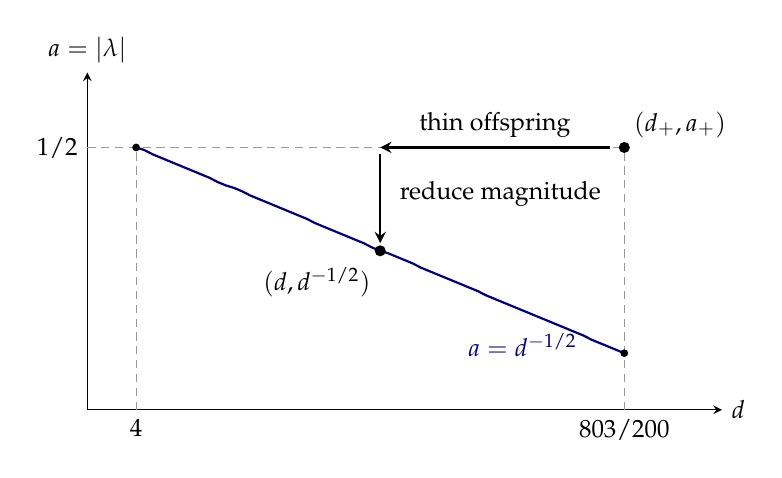
\begin{tikzpicture}[x=6.2cm,y=2.8cm,>=stealth,font=\small]
  \pgfmathsetmacro{\targety}{1000/sqrt(4+.015*.5)-499}
  \pgfmathsetmacro{\righty}{1000/sqrt(4+.015)-499}
  \draw[->] (-.10,-.19) -- (1.20,-.19) node[right] {$d$};
  \draw[->] (-.10,-.19) -- (-.10,1.34) node[above] {$a=|\lambda|$};
  \draw[densely dashed,black!40] (0,-.19) -- (0,1);
  \draw[densely dashed,black!40] (1,-.19) -- (1,1);
  \draw[densely dashed,black!40] (-.10,1) -- (1,1);
  \node[below] at (0,-.19) {$4$};
  \node[below] at (1,-.19) {$803/200$};
  \node[left] at (-.10,1) {$1/2$};
  \draw[thick,blue!50!black,domain=0:1,samples=61]
    plot (\x,{1000/sqrt(4+.015*\x)-499});
  \fill (0,1) circle (1.4pt);
  \fill (1,\righty) circle (1.4pt);
  \fill (1,1) circle (2pt);
  \node[above right] at (1,1) {$(d_+,a_+)$};
  \draw[->,thick] (.97,1) -- (.5,1)
    node[midway,above] {thin offspring};
  \draw[->,thick] (.5,.97) -- (.5,{\targety+.035});
  \node[right] at (.52,.79) {reduce magnitude};
  \fill (.5,\targety) circle (2pt);
  \node[below left] at (.5,{\targety-.03}) {$(d,d^{-1/2})$};
  \node[below right,text=blue!50!black] at (.66,.20)
    {$a=d^{-1/2}$};
\end{tikzpicture}
\caption{Domination in the first closed Poisson bin
$[4,803/200]$; the two axes use different enlarged scales.
The upper corner has $a_+=1/2$ and $d_+=803/200$, so it dominates
every equality experiment in the bin by thinning offspring and reducing
the channel magnitude.  It lies above the equality curve.
The certificate only brings its finite-depth upper law below $\mu=1/20$;
the local fixed-point gap is applied to the target equality experiment.}
\label{fig:dominating-bin}
\end{figure}

For each grid representative,
\[
 \left|\sum_i\frac{h_i}{H}\omega^i\right|^2
   =1-\frac{3(h_0h_1+h_1h_2+h_2h_0)}{H^2}.
\]
Define the integer
\begin{equation}
 M(m)=\sum_hm_h\bigl[H^2-3(h_0h_1+h_1h_2+h_2h_0)\bigr].
 \label{grid:moment}
\end{equation}
The certificate stops exactly when $20M(m)<NH^2$, equivalently
$\mu(m)<1/20$.  The exact code is included in
Section~\ref{cert:grid}.  With assertions enabled it returns iteration
$162$ for argument $-1$, the regular coloring recursion with four children at each vertex.
For arguments $j=0,\ldots,26$, the Poisson recursions return, in order,
\begin{equation}
\begin{gathered}
104,103,103,103,102,102,102,102,102,\\
101,101,101,101,101,101,\\
100,100,100,100,100,100,100,\\
99,99,99,99,99.
\end{gathered}
\label{grid:outputs}
\end{equation}
All comparisons determining these integers use exact integer arithmetic.
Appendix~\ref{grid:implementation} gives the bounds preventing overflow
and the correspondence between each code operation and the constructions
proved above.

\begin{proposition}[Completion of the negative threshold]
\label{grid:negative-completion}
For both tree models, every admissible negative parameter with
$da^2\leq1$ is non-reconstructible (with $d=b$ for a regular tree).
\end{proposition}
\begin{proof}
Consider first negative equality.  For the regular tree with $b=4$,
the upper law at depth $162$ has $\mu<1/20$.  For every Poisson
equality $d\in[4,881/200]$, choose a bin containing $d$ and its stopping
depth from~\eqref{grid:outputs}.  The corresponding upper law dominates
the exact equality depth experiment by the recursion and the two
garblings above.  Conditional Jensen gives
\mbox{$\mu_{\mathrm{true}}\leq\mu_{\mathrm{upper}}<1/20$} at that depth.
By Proposition~\ref{fnd:limit}, the actual depth laws have a symmetric
fixed-point limit and their moments decrease to its moment.  The limit
therefore has $\mu<1/20$ and is uniform by Proposition~\ref{loc:gap}.
This proves non-reconstruction in the certified range.

Proposition~\ref{fnd:limit} includes the coloring endpoint: its proof
extends the tilted recursion continuously across zero likelihood
normalizers and controls the Poisson count tail. Thus the preceding
fixed-point inference also applies at $a=1/2$.

Every remaining admissible regular equality has integer $b\geq5$ and
$a\leq1/\sqrt5<448/1000$.  Every remaining Poisson equality beyond
$881/200$ has $a<477/1000$ by~\eqref{grid:overlap}.
Proposition~\ref{wei:exclusion} excludes nonuniform fixed points in
these ranges, completing all negative equalities.

For $d\geq4$, every parameter $-d^{-1/2}\le\lambda<0$ is obtained by
the independent increment garbling from the equality parameter
$-1/\sqrt d$; hence its advantage also tends to zero.  For the remaining
parameters, first compare the coloring experiment with branching
parameter four to a smaller-branching coloring experiment.  For a
regular tree keep a fixed $b$ children at each vertex, and for a Poisson
tree retain each child with probability $d/4$, using the tree observation
and independent randomness.  This gives the smaller-tree observation
without the root.  Finally apply the increment garbling from $-1/2$ to
the desired negative parameter.  Thus all admissible negative channels
with branching parameter below four are non-reconstructible as well.
These are statements about the unconditional Poisson experiments, so
the conclusion uses exactly the averaging convention of the problem.
\end{proof}

\section{Completion and the stochastic block model}\label{sec:completion}
Table~\ref{tab:coverage} collects the arguments for the equality cases.
In the table, $a=|\lambda|$ denotes the negative channel magnitude.

\begin{table}[ht]
\centering\small
\begin{tabular}{@{}p{.21\textwidth}p{.36\textwidth}p{.34\textwidth}@{}}
\toprule
Equality case & Parameter range & Argument\\
\midrule
Positive channel & All admissible $d>1$ & Analytic exclusion, Section~\ref{sec:positive}\\
Negative, regular & $b\ge5$, so $a=b^{-1/2}<.448$ & Weighted identities, Section~\ref{sec:weighted}\\
Negative, regular & $b=4$, $a=1/2$ & Finite domination, Section~\ref{grid:section}\\
Negative, Poisson & $a=d^{-1/2}\le.477$ & Weighted identities, Section~\ref{sec:weighted}\\
Negative, Poisson & $4\le d\le881/200$ & Finite domination, Section~\ref{grid:section}\\
\bottomrule
\end{tabular}
\caption{Coverage of $d\lambda^2=1$, with $a=|\lambda|$ on the
negative side. The two Poisson ranges overlap since
$881/200>(1000/477)^2$. Below branching parameter four, negative channels
follow by degradation from the coloring case.}\label{tab:coverage}
\end{table}

\begin{proof}[Proof of Theorem~\ref{thm:threshold}]
Proposition~\ref{fnd:supercritical} proves reconstruction whenever
$d\lambda^2>1$.  Conversely, Proposition~\ref{pos:nonreconstruction}
proves non-reconstruction for $0\le\lambda\le d^{-1/2}$, and
Proposition~\ref{grid:negative-completion} proves it for every admissible
negative parameter with $d\lambda^2\le1$.  These conclusions include
all equality cases and exhaust the channel domain.  The Poisson
statements use the original tree law, without conditioning on survival.
\end{proof}

We return to the stochastic block model of Section~\ref{sec:sbm},
where $a,b>0$ are the within- and between-community connectivity
parameters and $d=(a+2b)/3>1$.  The remaining step is to apply the
external tree-to-graph and algorithmic results to the tree theorem.

\begin{proof}[Proof of Corollary~\ref{cor:sbm}]
Set
\[
 \lambda=\frac{a-b}{a+2b}\in(-1/2,1),\qquad
 d\lambda^2=\frac{(a-b)^2}{3(a+2b)}.
\]
The corresponding Poisson broadcast process has exactly the transition
matrix~\eqref{eq:channel}. Suppose first that $d\lambda^2\le1$.
Theorem~\ref{thm:threshold} gives $a_\ell\to0$ for this process.

To match the fixed-tree formulation of non-reconstruction, let $T$ be
the entire Poisson tree and put
\[
 A_\ell(T)=\E\!\left[
 \left\|\PP(\sigma_\rho=\cdot\mid T,\sigma_{\partial T_\ell})
       -\operatorname{Unif}\{1,2,3\}\right\|_{\mathrm{TV}}
 \mathrel{\Big|}T\right].
\]
For almost every fixed $T$, the boundary experiment is degraded as $\ell$
increases, so $A_\ell(T)$ decreases to a nonnegative limit $A_\infty(T)$.
The offspring beyond depth $\ell$ are independent of the root and
depth-$\ell$ spins conditional on $T_{\le\ell}$, and hence
$\E A_\ell(T)=a_\ell$. Bounded convergence therefore gives
$\E A_\infty(T)=0$, so $A_\infty(T)=0$ for almost every $T$.
If $\mu_{\ell,i}^T$ is the boundary law conditional on root state $i$
and $\overline\mu_\ell^T=\frac13\sum_i\mu_{\ell,i}^T$, Bayes' formula gives
\[
 A_\ell(T)=\frac13\sum_{i=1}^3
   d_{\mathrm{TV}}(\mu_{\ell,i}^T,\overline\mu_\ell^T),
\]
where $d_{\mathrm{TV}}$ denotes total-variation distance. The triangle inequality now shows that the pairwise total-variation
distances between the $\mu_{\ell,i}^T$ tend to zero for almost every $T$.
This is the non-reconstruction hypothesis of the tree-to-graph transfer
of Mossel, Sly, and Sohn \cite[Theorem~2.1]{MosselSlySohn2025}.
Their conclusion, with the overlap of their Definition~1.4, gives
\[
 \limsup_{n\to\infty}\E\operatorname{ov}(\sigma,\widehat\sigma_n)\le\frac13
\]
for deterministic estimators. Any violation by randomized estimators would,
for each $n$, admit a deterministic choice of the independent seed with
expected overlap at least the randomized expectation minus $1/n$,
contradicting the same bound. For every pair of labelings, the average
agreement over all six permutations is $1/3$, so its maximum is at least
$1/3$. This proves (i).

If $d\lambda^2>1$, Corollary~1 of Abbe and Sandon
\cite{AbbeSandon2018}, with three communities, gives an $O(n\log n)$
algorithm for detection. Their Lemma~1 converts their two-set detection
criterion, for uniform community probabilities, into overlap exceeding
$1/3$ by a fixed positive amount with probability tending to one.
This proves (ii).
\end{proof}

The corollary covers both $a>b$ and $a<b$. Its positive-parameter
hypothesis is part of the statement: the boundary cases $a=0$ or $b=0$
are not included. In particular, the negative equality has $d>4$ here;
the coloring equality $a=0$, $b=6$, $d=4$ is excluded.


\appendix
\section{The radial inequality}\label{rad:section}

This appendix proves the pointwise inequality used for positive channel
parameters.  Its algebraic certificates are given explicitly, so the proof
requires no numerical or computer-assisted verification.

\begin{lemma}[Radial inequality]\label{rad:lemma}
Let $m=(m_1,m_2,m_3)$ have positive coordinates and $\av{m}=1$, where
$\av{w}=\frac13\sum_{i=1}^3w_i$.  Put
\[
 v=m-1,\qquad x=\frac12\av{v^2},\qquad
 g=\av{\log m},\qquad u_i=\log m_i-g,
\]
\[
 J=\frac12\av{v\log m},\qquad B=\frac12\av{m u^2},
 \qquad F(m)=3g+4J+\frac45B.
\]
Since $I=g+2J$, this is the functional $F$ in
Equation~\eqref{pos:functional-F}. Then, for every $0<\lambda<1$,
\begin{equation}\label{rad:inequality}
 F(m)-\lambda^{-2}F(1+\lambda v)
 \geq \frac{1-\lambda^2}{2}\,x^2.
\end{equation}
\end{lemma}

\begin{proof}
Fix the message in the statement and
write
\[
 m(\tau)=1+\tau v^{(0)},\qquad x(\tau)=\tau^2x_0,
 \qquad \mathcal F(\tau)=F(m(\tau)),\qquad 0\leq\tau\leq1,
\]
where $v^{(0)}=m-1$ and $x_0=\frac12\av{(v^{(0)})^2}$.
Every coordinate of $m(\tau)$ is positive on this interval.
The functions are analytic near $\tau=0$.  Since $\av{v^{(0)}}=0$,
we have $g(\tau)=O(\tau^2)$, $J(\tau)=O(\tau^2)$ and
$B(\tau)=O(\tau^2)$, so $\mathcal F(\tau)=O(\tau^2)$.
Let $\partial=\tau\frac{d}{d\tau}$. We claim that it suffices to prove
\begin{equation}\label{rad:differential-bound}
 \partial(\partial-1)(\partial-2)\mathcal F(\tau)
 \geq12x(\tau)^2\qquad(0<\tau\leq1).
\end{equation}
To see this, suppose the bound holds along the ray.
Define
\[
 Y=(\partial-2)\mathcal F-x(\tau)^2,\qquad Z=(\partial-1)Y.
\]
The operator $\partial-2$ annihilates the quadratic Taylor term, giving
$Y=O(\tau^3)$ and $Z=O(\tau^3)$ as $\tau\downarrow0$.
Since $\partial(\partial-1)x(\tau)^2=12x(\tau)^2$,
Equation~\eqref{rad:differential-bound} gives $\partial Z\geq0$.
For $\tau>0$ this means $Z'(\tau)\geq0$, and $Z(0)=0$ therefore gives
$Z\geq0$.  Next,
\[
 \left(\frac{Y(\tau)}{\tau}\right)'
   =\frac{Z(\tau)}{\tau^2}\geq0.
\]
The limit of $Y(\tau)/\tau$ at zero is zero, so $Y\geq0$.  Finally,
\[
 \frac{d}{d\tau}
 \left[\frac{\mathcal F(\tau)-\tfrac12\tau^4x_0^2}{\tau^2}\right]
 =\frac{Y(\tau)}{\tau^3}\geq0.
\]
Evaluating the resulting monotonicity between $\tau=\lambda$ and $\tau=1$
gives
\[
 F(m)-\frac12x_0^2
 \geq\lambda^{-2}F(1+\lambda v^{(0)})
          -\frac12\lambda^2x_0^2,
\]
which is Equation~\eqref{rad:inequality}.

It remains to establish Equation~\eqref{rad:differential-bound} for every
positive message. All quantities in the following calculation refer to the
current message on the ray. Set
\[
 y=\frac12\av{v^3}.
\]
Thus $\partial v=v$, $\partial x=2x$, and $\partial y=3y$.
Introduce
\[
 U_j=\av{m^{-j}},\qquad S_j=\av{u m^{-j}},\qquad
 U=U_1,\quad S=S_1,\quad M=2J,\quad V=2B,\quad W=\av{u^2}.
\]
In particular $M=\av{m u}$, since $\av{u}=0$, and
$F=3g+2M+\frac25V$.  The identities
\[
 \partial\log m_i=1-m_i^{-1},\qquad
 \partial u_i=U-m_i^{-1}
\]
give
\begin{equation}\label{rad:differentiation}
\begin{aligned}
 \partial g&=1-U,&
 \partial M&=M+U-1,\\
 \partial V&=V-W+2UM,&
 \partial W&=-2S,\\
 \partial S&=U^2-U_2-S+S_2,&
 \partial U_j&=j(U_{j+1}-U_j).
\end{aligned}
\end{equation}
For example, differentiating $V=\av{m u^2}$ gives
$\av{v u^2}+2\av{m u(U-m^{-1})}=V-W+2UM$;
differentiating $S$ gives the next-to-last identity in
\eqref{rad:differentiation}.  Applying these identities to $F$ yields
\begin{equation}\label{rad:G}
\begin{aligned}
 G&:=\partial(\partial-1)(\partial-2)F\\
  &=6-12U+8U_2-2U_3\\
  &\quad+\frac45\bigl[S_2-3S+(2U_3-3U_2)M
                    +3(U-1)(U_2-U)\bigr].
\end{aligned}
\end{equation}
Our remaining goal is $G\geq12x^2$.

The elementary symmetric identities for the three zero-sum coordinates $v_i$
are
\begin{equation}\label{rad:cubic}
 v_i^3=3xv_i+2y,\qquad
 D_t:=\prod_{i=1}^3(1+t v_i)=1-3t^2x+2t^3y.
\end{equation}
Write $D=D_1$.  For $0\leq t\leq1$ all the factors in $D_t$ are positive
and have arithmetic mean one, so
\begin{equation}\label{rad:denominator-range}
 0<D_t\leq1.
\end{equation}
Define the coordinate polynomials
\[
 h_i=1-v_i+v_i^2-3x,\qquad
 k_i(t)=v_i-t(v_i^2-2x).
\]
The product of the two factors $1+v_j$ with $j\ne i$ is $h_i$, hence
$m_i^{-1}=h_i/D$.  Similarly, centering the logarithmic integral gives
\begin{equation}\label{rad:log-integral}
 \frac{v_i}{1+t v_i}-\av{\frac{v}{1+t v}}
   =\frac{k_i(t)}{D_t},\qquad
 u_i=\int_0^1\frac{k_i(t)}{D_t}\,dt.
\end{equation}
The first identity follows by multiplying by $D_t$ and using
\eqref{rad:cubic}; the second follows by integration.  All denominators here
are bounded away from zero for the fixed positive message under consideration.

Put $H_j=\av{h^j}$.  Substitution of these formulas into \eqref{rad:G}
separates its polynomial and logarithmic terms:
\begin{equation}\label{rad:RN-representation}
 D^3(G-12x^2)=R+\int_0^1\frac{N(t)}{D_t}\,dt,
\end{equation}
where
\begin{equation}\label{rad:RN-definition}
\begin{aligned}
 R={}&(6-12x^2)D^3-12H_1D^2+8H_2D-2H_3
       +\frac{12}{5}(H_1-D)(H_2-H_1D),\\
 N(t)={}&\frac45\av{k(t)
             \bigl[h^2D-3hD^2+(2H_3-3H_2D)v\bigr]}.
\end{aligned}
\end{equation}
In particular $N(t)$ is affine in $t$.  Let
\begin{equation}\label{rad:L-definition}
 L=R+\int_0^1N(t)(2-D_t)\,dt.
\end{equation}
Since
\[
 \frac1{D_t}-(2-D_t)=\frac{(1-D_t)^2}{D_t}\geq0,
\]
it suffices for \eqref{rad:differential-bound} to prove
\begin{equation}\label{rad:polynomial-goal}
 N(0)\geq0,\qquad N(1)\geq0,\qquad L\geq0.
\end{equation}
Indeed, the first two inequalities imply $N(t)\geq0$ on $[0,1]$, and then
\eqref{rad:RN-representation} is at least $L$.

We give the polynomial computations and their sign certificates in full.
For their verification one only needs the recurrence
\[
 P_0=1,\quad P_1=0,\quad P_2=2x,\qquad
 P_j=3xP_{j-2}+2yP_{j-3}\quad(j\geq3),
 \qquad P_j=\av{v^j}.
\]
The remaining moments that occur in \eqref{rad:RN-definition} are
\[
 P_3=2y,\quad P_4=6x^2,\quad P_5=10xy,\quad
 P_6=18x^3+4y^2.
\]
Expanding $h^j$ and using these moments gives
\begin{equation}\label{rad:H-expansions}
\begin{aligned}
 H_1&=1-x,\\
 H_2&=3x^2-4y+1,\\
 H_3&=-9x^3+9x^2+6xy+3x+4y^2-14y+1.
\end{aligned}
\end{equation}
The two coefficients of the affine polynomial $N(t)$ are explicitly
\begin{equation}\label{rad:N-expansion}
\begin{aligned}
 \frac5{24}N(t)={}&A(x,y)+t C(x,y),\\
 A(x,y)={}&3x^4+12x^3+x^2
   +(-6x^3-28x^2-2x)y+(26x-2)y^2-4y^3,\\
 C(x,y)={}&6x^4-2x^3
   +(-13x^3-10x^2-x)y+(10x^2+22x+4)y^2-16y^3.
\end{aligned}
\end{equation}
In particular their sum factors as
\begin{equation}\label{rad:N1}
 \frac5{24}N(1)=(x-y)(9x-10y+1)(x^2+x-2y).
\end{equation}
Integrating \eqref{rad:N-expansion} against $2-D_t$ in
\eqref{rad:L-definition}, and using \eqref{rad:H-expansions}, gives
\begin{equation}\label{rad:L-expansion}
\begin{aligned}
 \frac{25}{6}L={}&1500x^5-1020x^4+240x^3+168y^4\\
 &+(-480x^2-756x-52)y^3\\
 &+(2114x^3+710x^2+48x-80)y^2\\
 &+(-3093x^4+736x^3-35x^2)y.
\end{aligned}
\end{equation}
These are finite polynomial identities: the displayed moment recurrence
provides a direct way to check every coefficient.

We next describe the domain on which their signs are required.  Positivity
and $\sum_i m_i=3$ imply $\sum_i m_i^2<9$, and therefore $0\leq x<1$.
The discriminant identity for \eqref{rad:cubic} is
\[
 \prod_{1\leq i<j\leq3}(v_i-v_j)^2=108(x^3-y^2),
\]
so $|y|\leq x^{3/2}$.  Consequently each factor in \eqref{rad:N1} is
nonnegative, as is seen from
\begin{align*}
 x-y&\geq x(1-\sqrt{x}),\\
 9x-10y+1&\geq(1-\sqrt{x})(10x+\sqrt{x}+1),\\
 x^2+x-2y&\geq x(1-\sqrt{x})^2.
\end{align*}
This proves $N(1)\geq0$.

If $x=0$, then $v=0$ and the lemma is immediate, so henceforth take $x>0$.
Set $r=y/x$.  Then $r^2\leq x$ and $r\leq\sqrt{x}<1$, while $D>0$ gives
\begin{equation}\label{rad:domain}
 r^2\leq x<\frac1{3-2r}.
\end{equation}
The denominator is positive.  Combining these inequalities yields
\[
 0<1-r^2(3-2r)=(1-r)^2(2r+1),
\]
and hence $-\frac12<r<1$.  Every point of \eqref{rad:domain} is represented by
\begin{equation}\label{rad:z-substitution}
 x=\frac{r^2+z/(3-2r)}{1+z},\qquad y=rx,\qquad
 z=\frac{x-r^2}{1/(3-2r)-x}\geq0.
\end{equation}
Thus the parametrization includes $x=r^2$ without a limiting argument;
the excluded upper endpoint corresponds to a zero coordinate of $m$.

For clarity write $\widetilde N_0(r,z)$ and $\widetilde L(r,z)$ for $N(0)$
and $L$ after the substitution \eqref{rad:z-substitution}, and keep $x$
on the left sides below as the expression in that substitution.  The exact
coefficient identity for $N(0)$ is
\begin{equation}\label{rad:N0-certificate}
 (1+z)^2(3-2r)^2\frac{5\widetilde N_0}{24x^2}
   =a_0(r)+a_1(r)z+a_2(r)z^2,
\end{equation}
where
\begin{align*}
 a_0(r)&=(1-r)^3(3-2r)^2(10r^2+r+1),\\
 a_1(r)&=2(1-r)^3(3-2r)(9+5r+20r^2-4r^3),\\
 a_2(r)&=48(1-r)^3.
\end{align*}
All three coefficients are nonnegative for $-\frac12\leq r\leq1$.
For the first, the quadratic $10r^2+r+1$ has positive leading coefficient
and discriminant $1-40=-39<0$.  For the second,
\[
 9+5r+20r^2-4r^3=9+5r+r^2(20-4r)\geq\frac{13}{2}.
\]
The remaining factors in these expressions are visibly nonnegative.
Since the multiplier on the left of \eqref{rad:N0-certificate} is positive
on our domain, $N(0)\geq0$ follows.

The corresponding identity for $L$ is
\begin{equation}\label{rad:L-certificate}
 (1+z)^3(3-2r)^3\frac{25\widetilde L}{6x^2}
 =b_0(r)+b_1(r)z+b_2(r)z^2+b_3(r)z^3,
\end{equation}
where
\begin{align*}
 b_0(r)&=r^2(1-r)^3(3-2r)^3 f_0(r),\\
 b_1(r)&=(1-r)^3(3-2r)^2 f_1(r),\\
 b_2(r)&=2(1-r)^3(3-2r) f_2(r),\\
 b_3(r)&=24(1-r)^3(25-4r^2-10r),
\end{align*}
and every coefficient of the three remaining polynomials is as follows:
\begin{equation}\label{rad:f-polynomials}
\begin{aligned}
 f_0(r)&=480r^4-842r^3-117r^2+445r+160,\\
 f_1(r)&=336r^6-1008r^5+1096r^4-896r^3
                  +63r^2+685r+240,\\
 f_2(r)&=440r^4-1104r^3+368r^2+413r+210.
\end{aligned}
\end{equation}
Identities \eqref{rad:N0-certificate} and \eqref{rad:L-certificate}
follow by substituting \eqref{rad:z-substitution} into
\eqref{rad:N-expansion} and \eqref{rad:L-expansion}, respectively,
and clearing the displayed denominators.
The factor $25-4r^2-10r$ is at least $11$ on
$[-\frac12,1]$: its derivative is $-8r-10<0$ throughout that interval.
It remains to establish the signs of $f_0,f_1,f_2$.

Use the bijective change of variable
\[
 r=\frac{p-1/2}{1+p},\qquad
 p=\frac{r+1/2}{1-r}\geq0
 \quad\left(-\frac12\leq r<1\right).
\]
The resulting polynomial identities, with all coefficients displayed, are
\begin{equation}\label{rad:p-certificates}
\begin{aligned}
 4(1+p)^4 f_0\!\left(\frac{p-1/2}{1+p}\right)
    & =504p^4+4386p^3+12267p^2-1161p+174,\\
 4(1+p)^6 f_1\!\left(\frac{p-1/2}{1+p}\right)
    & =2064p^6+15486p^5+36669p^4+31368p^3\\
    &\qquad+20184p^2-2724p+522,\\
 4(1+p)^4 f_2\!\left(\frac{p-1/2}{1+p}\right)
    & =1308p^4+7650p^3+12366p^2-1842p+1044.
\end{aligned}
\end{equation}
Each right side is a polynomial with nonnegative coefficients in degrees
at least three, plus a strictly positive quadratic.  The exact
discriminants of those quadratic tails are
\begin{align*}
 (-1161)^2-4\cdot12267\cdot174&=-7\,189\,911<0,\\
 (-2724)^2-4\cdot20184\cdot522&=-34\,724\,016<0,\\
 (-1842)^2-4\cdot12366\cdot1044&=-48\,247\,452<0.
\end{align*}
Their leading coefficients are positive, so all three tails are strictly
positive on the real line.  Thus $f_i(r)>0$ for
$-\frac12\leq r<1$; their values at $r=1$ are, respectively,
$126,516,327$, also positive.  Every $b_j(r)$ is consequently nonnegative
on $[-\frac12,1]$.  Equation \eqref{rad:L-certificate} proves $L\geq0$,
finishing \eqref{rad:polynomial-goal} and hence
\eqref{rad:differential-bound}. The initial reduction now proves the lemma.
\end{proof}

\section{Correctness of the interval certificate}
\label{int:certificate}
\label{int:appendix}

This appendix explains the integer interval certificate for the strict
positivity of the polynomial~\eqref{wei:polynomial}.  The coefficients are
those in~\eqref{wei:coefficients}, with the matching parameter choices
in~\eqref{wei:parameters}.  The certified domain consists of every probability
vector on three states, every $\xi\in[3/100,1]$, and each of the three closed
$a$ intervals
\[
 [0,190/1000],\qquad [190/1000,448/1000],\qquad
 [448/1000,477/1000].
\]
The third interval uses the Poisson values $H=1/12$, $U=1/2$; the first
two use $H=1/16$, $U=15/32$.  The source is supplied unchanged as
\texttt{verification/interval.cpp}; see also
Section~\ref{cert:interval}.  Assertions and signed 128-bit integer
arithmetic are part of the certificate.  We first explain what its
arithmetic computes and then why normal completion proves the claimed
inequality over the entire domain.

\subsection{Coordinates, formulas, and boundary extensions}
\label{int:parametrization}

The quantities being checked are invariant under permutation of the
three coordinates.  After sorting a probability vector in decreasing
order, it has the representation
\begin{equation}
 p=\frac{(1,q^{18},r^{18})}{Z},\qquad
 Z=1+q^{18}+r^{18},\qquad 0\le r\le q\le1.
 \label{int:coordinates}
\end{equation}
Indeed, the largest probability is positive; take the eighteenth roots
of the other two probabilities divided by it.  The formulas below are
valid on the larger square $0\le q,r\le1$, which will allow rectangular
intervals that cross the diagonal $r=q$.

Set $m_i=3p_i$ and $v_i=m_i-1$.  Then
\[
 v=\left(\frac3Z-1,\frac{3q^{18}}Z-1,
                  \frac{3r^{18}}Z-1\right),\qquad
 x=\frac16\sum_{i=1}^3v_i^2,\qquad y=\frac12v_1v_2v_3.
\]
In particular, $-1\le v_i\le2$ everywhere on the square.  For positive
$q,r$, write $L_q=\log q$ and $L_r=\log r$.  The centered logarithms
$u_i=\log m_i-\frac13\sum_j\log m_j$ are
\[
 (-6(L_q+L_r),\ 12L_q-6L_r,\ 12L_r-6L_q).
\]
Consequently the functions used in the weighted argument are exactly
\begin{align}
 G&=\frac{3q^6r^6}{Z},& T&=1-G,\notag\\
 W&=\frac{216}{Z}q^6r^6(L_q^2+L_r^2-L_qL_r),\notag\\
 Y&=\frac{648}{Z}q^6r^6
    (2L_q^3+2L_r^3-3L_q^2L_r-3L_qL_r^2).
 \label{int:weighted-functions}
\end{align}
These expressions explain the constants $216$ and $648$ in
\texttt{coeff}.  The entries returned by \texttt{qt} are enclosures of
$q^{18}$ and $q^6(\log q)^j$, $0\le j\le3$, together with their
derivatives; the analogous entries are used for $r$.

For the edge functions put
\[
 e_i=1-av_i,\qquad G_e=(e_1e_2e_3)^{1/3},\qquad
 \mathcal L(t)=\begin{cases}-\log(1-t)/t,&t\ne0,\\1,&t=0.
 \end{cases}
\]
Define
\[
 b_i=-v_i\mathcal L(av_i),\qquad
 w_i=b_i-\frac13\sum_jb_j.
\]
For $a>0$, $b_i=\log(e_i)/a$, so the centered edge logarithms are
$aw_i$.  Since $\sum_i v_i=0$,
\[
 G_e^3=1-3a^2x-2a^3y.
\]
Factoring $1-G_e^3$ gives the formulas used in the code:
\begin{equation}
 \widehat T=\frac{3x+2ay}{1+G_e+G_e^2},\qquad
 \widehat W=\frac{G_e}{3}\sum_iw_i^2,\qquad
 \widehat Y=aG_ew_1w_2w_3.
 \label{int:edge-functions}
\end{equation}
Here $\widehat T=T_e/a^2$, $\widehat W=W_e/a^2$, and
$\widehat Y=Y_e/a^2$ when $a>0$.  The last identity uses
$\frac13\sum_iw_i^3=w_1w_2w_3$ for three centered coordinates.
Thus the code variables \texttt{Te}, \texttt{We}, and \texttt{Ye} are
the hatted quantities.  At $a=0$, the formulas give continuously
\[
 G_e=1,\qquad \widehat T=x,\qquad
 \widehat W=2x,\qquad \widehat Y=0.
\]
There is no division by $a$ in the implemented expressions.  Substituting
\eqref{int:weighted-functions} and~\eqref{int:edge-functions} into the
four entries returned by \texttt{coeff} gives, term by term,
$(D_0,D_1,D_2,D_3)$ in~\eqref{wei:coefficients}.  In the parameter
structure, \texttt{del}, \texttt{ch}, and \texttt{cu} mean
$\delta,H,U$, and the code forms $s_0=c_0+1/3$.

All boundary probability vectors are included.  Each function
$q^6(\log q)^j$, $0\le j\le3$, is assigned value zero at $q=0$.
Its derivative for $q>0$ is
\begin{equation}
 6q^5(\log q)^j+jq^5(\log q)^{j-1},
 \label{int:log-product-derivative}
\end{equation}
where the second term is omitted when $j=0$.  Both the function and
its derivative tend to zero at zero.  Thus the expressions have
continuous first derivatives up to the boundary; when $qr=0$ they give
$T=1$ and $W=Y=0$.  Since $Z\ge1$ and $e_i>0$ throughout the domain,
all four $D_i$ have the same regularity, including at $a=0$.

\subsection{Integer intervals and machine safety}
\label{int:arithmetic}

Let $S=2^{40}$.  An object \texttt{I} with integer endpoints $(l,h)$
represents $[l/S,h/S]$.  The functions \texttt{unit} and
\texttt{integer} represent a grid point and a small integer,
respectively.  With positive denominator, \texttt{rat}$(b,c)$ represents
\[
 \left[\frac{\lfloor Sb/c\rfloor}{S},
       \frac{\lceil Sb/c\rceil}{S}\right].
\]
The helpers \texttt{mf}$(b,c)$ and \texttt{floor\_div}$(b,c)$ compute
the mathematical floors of $bc/S$ and $b/c$, also for negative
numerators: the negative branch uses the negative of the corresponding
positive ceiling.  Upper endpoints are obtained by negating a floor of
a negated expression.  Addition and subtraction are exact on the
grid.  Multiplication chooses the appropriate endpoint extrema in
each sign case; when both intervals cross zero it takes the minimum
of the two potentially negative products and the maximum of the two
potentially positive products.  The square operation assigns lower
endpoint zero when its input crosses zero.

For a positive interval $[l/S,h/S]$, the reciprocal is enclosed by
\[
 \left[\frac{\lfloor S^2/h\rfloor}{S},
       \frac{\lceil S^2/l\rceil}{S}\right].
\]
Negative reciprocals use odd symmetry.  An assertion excludes intervals
containing zero.  Consequently all elementary interval operations
contain their exact real counterparts.  Intersecting a value interval
with a separately established range is also sound.  The two uses of
this operation, \texttt{clip}, are the range $[-1,2]$ for $v_i$ and
the logarithmic-product bounds proved below.

These statements concern exact integer operations, so absence of
overflow must be established before using their outputs.  Every
potentially growing endpoint calculation is passed through
\texttt{safe}, which asserts
\[
 -2^{62}<b<2^{62}
\]
before converting the signed 128-bit integer $b$ to a signed 64-bit
endpoint.  Inductively, two input endpoints have product of magnitude
less than $2^{124}$.  The product is formed after promoting to signed
128 bits, and the rounding offset $S-1$ still leaves its magnitude
below $2^{127}$.  Endpoint addition is also promoted before checking.
Reciprocal numerators are $S^2=2^{80}$; adding the denominator minus
one for upward rounding is safe.  Rational-construction numerators
and denominators in the prescribed runs are small fixed integers.
No unchecked negation or absolute value can encounter the minimum
signed 64-bit integer, because endpoints have magnitude below $2^{62}$.

The remaining raw integer expressions have separate small bounds.
All box coordinates lie in $[0,S]$ in grid units, so midpoint sums
are at most $2S$.  Cube-root search candidates are below $2S$,
their endpoint sums are at most $4S$, and the two cube-comparison
operands are below $8S^3=2^{123}$.  The fixed multiples of $S$, loop
indices, and initial-grid numerators fit signed 64 bits.
The unchecked visit counter is treated separately by the concrete
sanitized executions recorded below; the depth bound alone does not
keep its total number of increments within the signed 64-bit range.
Logarithm scaling uses at most forty doublings on the actual
arguments.  Thus a range assertion is never being asked to detect an
overflow that has already occurred: oversized derivative or value
enclosures stop at \texttt{safe} before narrowing.  All floating-point
casts in this source occur in failure diagnostics, not in acceptance
tests.

\subsection{Logarithms, divided logarithms, and cube roots}
\label{int:logs}

The function \texttt{atanh2} evaluates the fifteen terms
\[
 2\sum_{n=0}^{14}\frac{w^{2n+1}}{2n+1}
\]
by Horner's rule with outward interval operations.  For $|w|\le u<1$
the absolute remainder is at most
\[
 \frac{2u^{31}}{31(1-u^2)}.
\]
The code asserts $|w|\le1/3+4/S<3/8$.  With $u=3/8$, the remainder
bound, in grid units, is the exact rational number
\begin{equation}
 S\frac{2(3/8)^{31}}{31(1-(3/8)^2)}
 =\frac{617673396283947}{119978708822917120}
 <\frac1{100}<2.
 \label{int:atanh-tail}
\end{equation}
The padding $[-2/S,2/S]$ therefore covers the omitted tail; all
polynomial-evaluation errors are already covered by interval rounding.

To enclose $\log(x/S)$ for a positive integer endpoint $x$,
\texttt{ln} scales an interval containing $x/S$ by powers of two.
If $m$ is the resulting interval and $k$ the accumulated exponent,
then $x/S\in2^km$.  Multiplication by two is exact on this grid;
halving, when used, rounds outwards.  The identities
\[
 \log t=2\operatorname{atanh}\frac{t-1}{t+1},\qquad
 \log2=2\operatorname{atanh}\frac13
\]
give the enclosure after adding $k\log2$.  The domain assertion in
\texttt{atanh2} checks the needed range even after rounding.  All
positive arguments actually passed to \texttt{ln} are either coordinate
endpoints in $[1/S,1]$, or endpoints of $1-av_i$ bounded away from
zero, so the scaling loops terminate within the stated bounds.

The divided logarithm has the integral and power-series representations
\begin{equation}
 \mathcal L(t)=\int_0^1\frac{ds}{1-st}
             =\sum_{n=0}^{\infty}\frac{t^n}{n+1}
 \quad (|t|<1).
 \label{int:L-representation}
\end{equation}
For $|t|\le1/4$, \texttt{L\_endpoint} evaluates
$\sum_{n=0}^{22}t^n/(n+1)$ and its derivative
$\sum_{n=1}^{22}nt^{n-1}/(n+1)$ independently.  Bounding both
coefficient sequences by one bounds their absolute tails by
\begin{equation}
 \frac{(1/4)^{23}}{1-1/4}=\frac1{48S},\qquad
 \frac{(1/4)^{22}}{1-1/4}=\frac1{12S},
 \label{int:L-tails}
\end{equation}
respectively.  Each receives padding $[-1/S,1/S]$.  Outside this
small interval the exact identities
\[
 \mathcal L(t)=-\frac{\log(1-t)}t,\qquad
 \mathcal L'(t)=\frac{(1-t)^{-1}-\mathcal L(t)}t
\]
use only nonzero denominators.  On the entire real domain $t<1$,
differentiation of the integral representation gives
\[
 \mathcal L'(t)=\int_0^1\frac{s\,ds}{(1-st)^2}>0,\qquad
 \mathcal L''(t)=2\int_0^1\frac{s^2\,ds}{(1-st)^3}>0.
\]
Thus both $\mathcal L$ and $\mathcal L'$ increase, including at negative
arguments.  The lower enclosure at the left endpoint and upper
enclosure at the right endpoint suffice to enclose each function
on an interval.  This is precisely the rule used by \texttt{L}.

For a nonnegative integer $x<8S$, \texttt{cb\_floor} uses binary
search and the exact comparison
\[
 m^3\le xS^2
\]
to return $\lfloor S(x/S)^{1/3}\rfloor$.  Its initial search bracket
$[0,2S]$ is valid by $x<8S$.  Applying this function to the two input
endpoints, then increasing the upper result by one grid unit, encloses
the cube root.  The derivative enclosure is obtained from
$1/(3t^{2/3})$ using the already enclosed positive root.

The outward rounding of an $a$ endpoint enlarges the prescribed bands
by less than $1/S$, and never introduces negative $a$.  Hence throughout
the actual boxes $a\le477/1000+1/S$.  Even the interval enclosures of
$1-av_i$, after multiplication rounding and clipping $v_i$ to $[-1,2]$,
have lower endpoint greater than $45/1000$ and upper endpoint less
than $1478/1000$.  The successive product of the three factors has
lower endpoint at least $(45/1000)^3-3/S>0$ and upper endpoint at most
$(1478/1000)^3+3/S<8$.  These bounds justify the logarithm,
divided-logarithm, reciprocal, and cube-root domains on every initial
box and descendant.  The cube-root lower enclosure is positive as
well, so its derivative reciprocal is valid.

\subsection{Logarithmic products and derivative propagation}
\label{int:derivatives}

The zero endpoints in~\eqref{int:coordinates} are treated without
evaluating their logarithms.  For $0<q\le1$, set $t=-\log q\ge0$.
For integers $0\le j\le3$ and real $h\ge5$,
\[
 q^{h/2}|\log q|^j=e^{-ht/2}t^j\le1.
\]
For $j=0$ this is immediate.  For $j>0$ its maximum is
$(2j/(he))^j\le1$, since $2j/h\le6/5<e$.
It follows that
\begin{equation}
 |q^5(\log q)^j|\le q^{5/2}\le q^2,\qquad
 |q^6(\log q)^j|\le q^3.
 \label{int:qt-bound}
\end{equation}
For even $j$ the products are nonnegative, and for odd $j$ they are
nonpositive.  These are the exact external ranges used by
\texttt{qt\_direct} to intersect the power-and-logarithm enclosures.
When the lower endpoint is zero, the same ranges directly supply
an enclosure, with no logarithm call.  When the lower endpoint is
positive, monotonicity of $\log$ supplies its interval, and intersecting
its upper bound with $0$ is valid because $q\le1$.  The derivative
returned for every logarithmic product is exactly the interval
version of~\eqref{int:log-product-derivative}.  The derivative of
$q^{18}$ is $18q^{17}$.  Cached enclosures depend only on the interval
endpoints; \texttt{qt} puts their derivatives in the appropriate
$q$ or $r$ gradient coordinate.

An object \texttt{J} consists of a value interval and three derivative
intervals, corresponding to $(q,r,a)$.  Constants have zero gradients
and variables have the appropriate unit gradient.  Addition,
multiplication, squares, and reciprocals apply the identities
\[
 \partial_i(fg)=f\,\partial_i g+g\,\partial_i f,\qquad
 \partial_i(f^2)=2f\,\partial_i f,\qquad
 \partial_i(f^{-1})=-f^{-2}\partial_i f.
\]
Cube roots and $\mathcal L$ use the derivative enclosures just proved
and the chain rule.  Induction over these operations proves that the
value and every first partial derivative of the actual formula are
enclosed throughout the box.  Tightening a value enclosure by an
external range does not replace the underlying function by a clipped
function: its previously enclosed derivatives remain valid, and
the tighter values can be used in subsequent product and chain rules.
All these statements extend to zero coordinate endpoints by the
continuous derivative extensions already established.

\subsection{Bernstein coefficients and the acceptance test}
\label{int:bernstein}

For fixed $(q,r,a)$ write the polynomial as
$P(\xi)=D_0+D_1\xi+D_2\xi^2+D_3\xi^3$.  On a subinterval
$[l,h]$, substitute $\xi=l+(h-l)t$, $0\le t\le1$, and express $P$
in the basis $\binom3j t^j(1-t)^{3-j}$.  The multipliers of $D_1,D_2,D_3$
in the four coefficients are
\begin{equation}
 \begin{array}{c|ccc}
 j& D_1&D_2&D_3\\ \hline
 0&l&l^2&l^3\\
 1&(2l+h)/3&l(l+2h)/3&l^2h\\
 2&(l+2h)/3&h(h+2l)/3&lh^2\\
 3&h&h^2&h^3
 \end{array}
 \label{int:bernstein-rows}
\end{equation}
and the multiplier of $D_0$ is always one.  Expanding the four
basis polynomials verifies these identities.  All basis polynomials
are nonnegative and their sum is one; strictly positive coefficients
therefore imply $P(\xi)>0$ on the whole closed subinterval.

The function \texttt{rows} uses successive intervals with endpoints
\begin{equation}
 \frac1{1000}(30,50,75,100,150,200,300,400,500,650,800,900,1000).
 \label{int:xi-grid}
\end{equation}
These twelve intervals cover $[3/100,1]$ without gaps.  For each it
stores the first three rows of~\eqref{int:bernstein-rows}; the fourth
row equals the first row for the next interval.  It finally adds
$(1,1,1)$.  Thus the $37$ stored rows account for all $48$ coefficients
of the twelve cubic representations, including both extreme
endpoints.  The row multipliers are themselves evaluated by rational
interval arithmetic and have zero gradients with respect to
$(q,r,a)$.

Let $F$ denote one of these Bernstein coefficients on a box
$B=\prod_{i=1}^3[l_i/S,h_i/S]$.  The interval calculation in
\texttt{dot} encloses $F$ and all its first derivatives.  A positive
lower endpoint immediately accepts this coefficient.  Otherwise
define the grid midpoint and coordinate radii by
\[
 c_i=\frac{\lfloor(l_i+h_i)/2\rfloor}{S},\qquad
 \rho_i=\frac{h_i-\lfloor(l_i+h_i)/2\rfloor}{S}.
\]
Nonnegative endpoints ensure that C++ integer division computes this
floor; $\rho_i$ is the larger of the two distances to the endpoints.
If $M_i$ is the maximum absolute endpoint of the derivative enclosure,
in real units, then for every $z\in B$ the segment from $c$ to $z$
lies in $B$ and
\begin{equation}
 F(z)\ge F(c)-\sum_{i=1}^3M_i\rho_i.
 \label{int:mean-value}
\end{equation}
This follows by integrating the gradient along that segment, also
when a coordinate endpoint is zero.  The code encloses $F(c)$ anew,
rounds each product $M_i\rho_i$ upwards, and adds their integer
upper endpoints with overflow checks.  Its strict comparison
\texttt{value.v.l > total} is therefore sufficient for $F>0$
throughout $B$.  A box is accepted only when every stored row passes
one of these two tests.

\subsection{Subdivision, coverage, and observed completion}
\label{int:coverage}

For a band $[a_-,a_+]$, the initial exact boxes before outward
rounding are
\begin{equation}
 \left[\frac i{24},\frac{i+1}{24}\right]
 \times\left[\frac j{24},\frac{j+1}{24}\right]
 \times\left[a_-+\frac{k}{16}(a_+-a_-),
              a_-+\frac{k+1}{16}(a_+-a_-)\right],
 \label{int:initial-boxes}
\end{equation}
where $0\le i<24$, $0\le j\le i$, and $0\le k<16$.
Every $(q,r)$ with $0\le r\le q\le1$ belongs to one of the displayed
$q,r$ rectangles, including all grid boundaries.  There are
$16\sum_{i=0}^{23}(i+1)=4800$ initial boxes per run.  Their endpoints
are rounded outwards, so none of the required domain is lost.
The extra points included by rounding are harmless, as are portions
of diagonal rectangles with $r>q$: the same functions and derivative
bounds are valid there.  The $a$ enlargement and all analytic domains
were checked above.  Adjacent bands may use different parameters,
since each certifies its own entire closed band.

On entry, \texttt{visit} skips a box only if its lower $r$ endpoint
exceeds its upper $q$ endpoint.  Such a box contains no point with
$r\le q$.  If any coefficient fails both acceptance tests, the code
chooses a coordinate with maximal recorded derivative-radius
contribution and cuts at its grid midpoint.  The choice affects
efficiency only.  The two closed children include the midpoint and
their union is the parent.  If the chosen contribution is zero, the
depth exceeds $80$, or the chosen grid radius is at most one, an
assertion fails rather than accepting an unresolved box.

Induction back up any normally completed recursion tree now proves
that every required point in its root box has all Bernstein
coefficients strictly positive.  The leaves either pass the sound
acceptance tests or contain no required point.  Together with
\eqref{int:initial-boxes}, \eqref{int:xi-grid}, and the sorted
parametrization, normal completion of all three runs proves the
pointwise inequality on the full stated domain.  This includes the
uniform message, boundary probability vectors, $a=0$, all band
endpoints, and all $\xi$ endpoints.  In particular there is no
exception at the uniform message: there $P(\xi)=\delta\xi^2+
U\delta\xi^3>0$.

\label{int:execution}
The unchanged source was replayed with GCC 13.3.0 on x86\_64 Linux,
using assertions enabled.  From the package root the reproduction
commands are
\begin{verbatim}
g++ -std=c++17 -O3 -UNDEBUG verification/interval.cpp \
  -o /tmp/appendix_b
/tmp/appendix_b 0
/tmp/appendix_b 1
/tmp/appendix_b 2
\end{verbatim}
Only the documented arguments $0,1,2$ are part of this protocol;
the source does not validate other argument values.  Compiling with
assertions disabled is not this certificate.  All three runs exited
normally with status zero and the following visit counts:
\[
 \begin{array}{c|c|r}
 \text{argument}&a\text{ interval}&\text{calls to \texttt{visit}}\\ \hline
 0&[0,190/1000]&414080\\
 1&[190/1000,448/1000]&756096\\
 2&[448/1000,477/1000]&1004426
 \end{array}
\]
The counts include internal subdivision nodes and boxes skipped by
the diagonal test. All three executions were also repeated on the
unchanged source with \texttt{-O2 -UNDEBUG -fsanitize=undefined}
and \texttt{-fno-sanitize-recover=undefined}. They completed with the
same counts and no sanitizer diagnostics. This supplies the separate
check of the unchecked \texttt{visits++} counter for these prescribed
executions. The counts identify the finite completed executions;
their correctness implication is the enclosure and coverage argument
above, not a sample-based inference.  The source SHA-256 is
\begin{verbatim}
76d1443b1194597ee77749e8030c825f2b9aae46b5c172d9eccf0745078c28e3
\end{verbatim}

\section{Exact arithmetic and reproduction of the grid certificate}
\label{grid:implementation}

The complete C++17 program in Section~\ref{cert:grid} implements the
recursions of Section~\ref{grid:section}.  Its parameters are fixed at
$H=72$, $N=10^{12}$, and $\mathtt{SCALE}=10^{15}$.  It uses signed
64-bit integers for table coefficients and mass units, and signed
128-bit integers for products and accumulators. The compiler must also
provide a plain \texttt{int} type of at least 32 bits. Assertions must be
enabled; in particular the build must not define \texttt{NDEBUG}.
For example, from the paper directory, the following commands compile and run all 28 cases:
\begin{verbatim}
g++ -std=c++17 -O3 -UNDEBUG -Wall -Wextra \
    verification/grid.cpp -o grid
for j in $(seq -1 26); do ./grid "$j"; done
\end{verbatim}
The program writes progress diagnostics to standard error and the case
number followed by its stopping iteration to standard output.  Only
the diagnostics convert to floating point.  Successful outputs are
specified in~\eqref{grid:outputs}, together with \texttt{-1 162}.

\subsection{Correspondence of code and probability operations}

The routine \texttt{init} enumerates all sorted nonnegative integer
triples of sum $72$.  It finds $469$ triples, identifies the pure
representative $(72,0,0)$ and the uniform representative $(24,24,24)$,
and stores an index for every representative.  The routine
\texttt{indexof} sorts a candidate triple and verifies the resulting
index.  A \texttt{Law} is a vector of orbit masses in units of $1/N$.
The routine \texttt{complete} adds the missing units at the pure orbit,
which is exactly Lemma~\ref{grid:completion}.

The constructor \texttt{Table(mode,A,AD)} first reduces the channel
fraction.  The variables \texttt{lhs}, \texttt{rhs}, \texttt{raw},
\texttt{T}, and \texttt{den} are the entries and denominator of
\eqref{grid:modes}.  For each of the six relative permutations,
\texttt{n}, \texttt{rem}, and \texttt{miss} are the floor vector,
remainders, and deficit in the grid spread.  The corner weights are
\texttt{T}, \texttt{rem[c]}, or \texttt{T-rem[c]}, as appropriate.
After aggregating equal output indices, the constructor checks that
their sum is \texttt{den}.  These checks include every grid pair, not
only pairs visited by an iteration.  Zero normalizers are omitted
because they have zero tilted mass.

The routine \texttt{combine} implements~\eqref{grid:combine}.  Symmetric
modes use the triangular pair table and the stated off-diagonal
coefficient; mode~1 uses ordered pairs.  Its row-skipping condition is
safe: an ordered row contributes zero when its first mass is zero,
while a triangular row contributes zero when both first-index masses
are zero.  The table position advances by the full skipped row length.
After division by $N\,\mathtt{den}$, each mass is rounded down and
\texttt{complete} is applied.

The functions \texttt{down} and \texttt{up} compute floor and ceiling
of a nonnegative integer ratio.  The latter uses
$\lceil x/y\rceil=\lfloor(x+y-1)/y\rfloor$ for $x\geq0$, $y>0$.
The function \texttt{w\_zero} implements~\eqref{grid:taylor}.
The routine \texttt{poisson} fixes its incoming child law
\texttt{inc}, starts \texttt{part} at the uniform zero-count law, and
uses mode~1 once for each positive count weight.  Its orbit sums are
exactly~\eqref{grid:mixture}; the final \texttt{complete} handles all
omitted mass.  No count product is needed after the first zero weight.
The regular branch of \texttt{run} is~\eqref{grid:regular-recursion}.
Finally, \texttt{mu\_num} is $M$ in~\eqref{grid:moment}, and the strict
stopping test is $20M<NH^2$.  Each run allows $400$ iterations and
asserts failure if none succeeds.  All reported stopping iterations
are below that bound.

\subsection{Bounds on every arithmetic class}

For all Poisson table calls, the reduced fraction satisfies
$B\leq10^6$ and $A\leq B/2$.  Thus
\[
 0\leq e_i\leq(B+A)H\leq108000000,
 \quad D_{\mathrm{tab}}=6BH^2\leq31104000000,
 \quad Hr_i\leq559872000000.
\]
Each total $T$ is at most three times the bound on a raw coordinate;
all of these quantities fit signed 64 bits.  The only mode~2 call is
at the reduced fraction $A/B=1/2$, where
$D_{\mathrm{tab}}=373248$ and $Hr_i\leq3359232$.
Mode~0 has smaller bounds.  Every nonnegative aggregated table weight
and every partial sum of weights is bounded by its denominator, by
\eqref{grid:table-mass}.

Input masses are nonnegative and sum to $N$, so their ordered pair
mass is $N^2$.  The triangular implementation has the same total
after the off-diagonal terms are combined.  Consequently every
nonnegative product accumulator and its partial sums are at most
\[
 D_{\mathrm{tab}}N^2
 \leq31104000000000000000000000000000000<2^{127}-1.
\]
The source casts an input factor to the 128-bit type \texttt{Big}
before multiplying.  Dividing by $ND_{\mathrm{tab}}$ yields a mass
between zero and $N$, safely convertible back to 64 bits.  The
uncompleted masses sum to at most $N$; likewise the Poisson mixture
masses sum to at most $N$, since they are lower bounds on a probability
mixture.  These facts bound all 64-bit partial sums in
\texttt{complete} and \texttt{poisson}.

Here are bounds for the Taylor calculation independent of machine
floating point.  If $t_n=S_0d_+^n/n!$, the lower and upper endpoint
errors satisfy
\[
 0\leq t_n-l_n< e^{d_+},\qquad
 0\leq u_n-t_n< e^{d_+}.
\]
Indeed an error satisfies $\epsilon_n\leq(d_+/n)\epsilon_{n-1}+1$;
expanding this recurrence bounds it by
$\sum_{j\geq0}d_+^j/j!=e^{d_+}$, since each product of $j$ successive
denominators is at least $j!$.  As $d_+<5$ and $e<3$, the endpoint
errors are less than $243$.  The sum of all endpoint magnitudes through
degree $41$ is therefore bounded by
\[
 S_0e^{d_+}+42\cdot243<243(S_0+42)<2^{63}-1.
\]
This also bounds every signed partial sum in~\eqref{grid:taylor}.
The endpoint multiplication by $d_{\max}\leq881$ is carried out in
128 bits before division, and the same holds for multiplication by
$N$ and for the Poisson weight recurrence.  These products are all
less than $2^{127}-1$ under the displayed bounds.

The lower sum $L$ is positive.  In fact Taylor's theorem gives
\[
 \frac{L}{S_0}
 \geq e^{-d_+}-\frac{d_+^{42}}{42!}
                   -\frac{41\cdot243}{S_0}
 >\frac1{243}-10^{-20}-\frac{9963}{10^{15}}>0.
\]
The middle inequality uses the elementary integer comparison
$5^{42}/42!<10^{-20}$.  Thus the nonnegative-argument conditions of
\texttt{down} hold at the final Taylor step as well as in its term
recurrences. Since $w_n/N\leq p_n$, every Poisson weight is at most
$N$. In particular $w_8\leq N<2^{40}$, and the recurrence gives
$w_n\leq w_{n-1}/2$ for $n\geq9$, since $d_+/n<1/2$.
Thus $w_{48}<1$, so the first zero occurs by $n=48$. The count loop
and its denominator therefore satisfy $n\leq48$ and $200n\leq9600$,
well within the plain integer type. Every product $w_nq_n(h)$ is at
most $N^2$ and is evaluated in 128 bits.

For $h\in\mathcal H$, the bracket in~\eqref{grid:moment} belongs to
$[0,H^2]$.  Hence every partial sum in \texttt{mu\_num} is at most
\[
 NH^2=5184000000000000<2^{63}-1.
\]
The factor $20$ in the stopping comparison is applied after converting
to \texttt{Big}.  The binary-search comparisons for~\eqref{grid:magnitude}
likewise use 128 bits before taking integer squares and products.

There are at most $18$ unaggregated contributions per grid pair
(six permutations, at most three corners).  Thus even a full ordered
table has at most $18\cdot469^2=3959298$ entries before aggregation.
All table positions and vector indices fit an ordinary signed 32-bit
integer, and the source also checks an explicit
$100000000$ entry limit.  Candidate grid coordinates belong to
$\{0,\ldots,H\}$, and all small grid sums and products fit these
integer types.  This accounts for the unguarded indexing arithmetic
as well as the probabilistic accumulators.

The supplied source therefore implements a finite exact-arithmetic
certificate: positivity, normalization, rounding direction, all
parameter choices, and the final strict inequalities are independent
of compiler floating-point behavior.

\section{Exact verification programs}\label{app:certificates}
The three programs below are part of the proof. They use integer or
rational arithmetic for every certification decision. In the C++ programs,
floating-point conversion is used only for diagnostic output.
The mathematical meaning and arithmetic guarantees of the programs are
proved in Sections~\ref{sec:local}--\ref{sec:weighted},
Section~\ref{grid:section}, and
Appendices~\ref{int:appendix} and~\ref{grid:implementation}, and in
the pair derivation below.

\subsection*{Reproduction protocol}
The accompanying directory \texttt{verification/} contains
\texttt{pair.py}, \texttt{interval.cpp}, and \texttt{grid.cpp},
exactly the sources printed below. Run Python with SymPy installed
and with assertions enabled. Compile the C++ sources with a compiler
supporting signed \texttt{\_\_int128} and a plain \texttt{int} type of
at least 32 bits, also with assertions enabled.
For example, from the paper directory:
\begin{lstlisting}[numbers=none]
python verification/pair.py
g++ -std=c++17 -O3 -UNDEBUG verification/interval.cpp -o interval
g++ -std=c++17 -O3 -UNDEBUG verification/grid.cpp -o grid
for j in 0 1 2; do ./interval "$j"; done
for j in -1 $(seq 0 26); do ./grid "$j"; done
\end{lstlisting}
Do not use Python's \texttt{-O} option, and do not define \texttt{NDEBUG}.
Only the displayed argument ranges are part of the protocol.
The bundled runner \nolinkurl{verification/reproduce.py} verifies the source
hashes, runs this suite, checks the expected outputs, and saves the
commands, software versions, exit statuses, and logs in its designated
output directory. Its usage is documented in the accompanying README.

Successful execution of the pair program produces no output.
The interval runs finish with visited-box counts
$414080$, $756096$, and $1004426$, respectively.
The grid run with argument $-1$ stops at iteration $162$.
The other grid stopping iterations are recorded in
Section~\ref{grid:section}.
The certificate sources were replayed with Python~3.12.13,
SymPy~1.14.0, and GCC~13.3.0 on x86\_64 Linux; all 32 mathematical
executions and five environment/compiler checks passed. Separately, the
three interval cases were replayed with \texttt{-O2 -UNDEBUG},
\texttt{-fsanitize=undefined}, and
\texttt{-fno-sanitize-recover=undefined}. All three exited successfully,
with the same progress logs and no sanitizer diagnostics. This supplemental
check is distinct from the ordinary runner protocol and supplies the
execution check on the visit counter discussed in
Appendix~\ref{int:appendix}.

The SHA-256 digests of the three source files, in the above order, are
\begin{quote}\small\ttfamily
\nolinkurl{ab775c3a63fb1d2713bfe058af2dece4ceda99627c17ce18f51f817b69410bba}\\
\nolinkurl{76d1443b1194597ee77749e8030c825f2b9aae46b5c172d9eccf0745078c28e3}\\
\nolinkurl{03c92321efedd0db53b1e91372918dfcd68d459db0223cb160c39df3bd645283}
\end{quote}
These digests identify the exact files; the correctness arguments are
provided in the text, and the successful runs establish the finite
assertions required there.

\subsection{Pair coefficient certificate}\label{cert:pair}
We prove the $a=1/2$ case of Lemma~\ref{loc:pair} for strictly
positive input vectors, using its notation for the input invariants and
pair excesses.  The main-text proof then extends these bounds to every
$0\le a\le1/2$ and to the closed simplex.
Parametrize sorted unnormalized vectors by
\[
 p=(6s+3t+2,3t+2,2),\qquad
 q=(6u+3v+2,3v+2,2),\qquad s,t,u,v\ge0.
\]
This covers every strictly positive sorted vector up to scale: for
$h_0\ge h_1\ge h_2>0$, take
$s=(h_0-h_1)/(3h_2)$ and $t=2(h_1-h_2)/(3h_2)$ to obtain
$p=2h/h_2$.  Put $P=\sum_i p_i$, $Q=\sum_i q_i$, and
$e_i=Q-q_i$, with $E=\sum_i e_i=2Q$.  Then
$e_i/E=(1-q_i/Q)/2$, as required for the coloring edge.
For an unnormalized vector $r$ of total $R$, put
\[
 N_x(r)=\frac{3\sum_i r_i^2-R^2}{2},\qquad
 N_y(r)=\frac{27\prod_i r_i-R^3+3R N_x(r)}2.
\]
The identities for the posterior invariants give
$N_x(r)=R^2x(r/R)$ and $N_y(r)=R^3y(r/R)$.
These are the two numerators returned by \texttt{xy} in the source.

For each of the two choices
$\widetilde e=(e_0,e_1,e_2)$ and $\widetilde e=(e_0,e_2,e_1)$,
let
\[
 r_i^{(j)}=p_i\widetilde e_{i+j},\qquad
 T_j=\sum_i r_i^{(j)},\qquad j=0,1,2,
\]
with indices modulo three.  The likelihood normalizer is
$3T_j/(PE)$; multiplying by the cyclic probability $1/3$ gives weight
$T_j/(PE)$.  Since $\sum_jT_j=PE$, these are probability weights.
The two choices, each followed by the three rotations, enumerate all
six relative permutations.  Repeated representatives at a stabilizer
remain valid uniform group averages.

For each reflection class separately, clear the positive denominator
\begin{equation}\label{loc:denominator}
 D=PE(T_0T_1T_2)^3P^4E^4.
\end{equation}
The three expressions \texttt{out[0]}, \texttt{out[1]}, and
\texttt{out[2]} divided by $D$ are exactly
\[
 \sum_{j=0}^2\frac{N_x(r^{(j)})}{PE T_j},\qquad
 \sum_{j=0}^2\frac{N_y(r^{(j)})}{PE T_j^2},\qquad
 \sum_{j=0}^2\frac{N_x(r^{(j)})^2}{PE T_j^3},
\]
namely the tilted output means of $x,y,x^2$ within that class.
For every call in the source,
\[
 \frac{\texttt{mon}(i,j,k,l)}D=X^i y_0^j z^kB_0^l.
\]
The powers $4-2i-3j$ and $4-2k-3l$ in these calls are nonnegative,
so the cleared objects are polynomials.  Hence \texttt{dx},
\texttt{de}, and \texttt{dn} are $D$ times the class-specific excesses.

The correction \texttt{im}, after division by $D$, is
\begin{equation}\label{loc:reflection}
 I=\frac{27\,\operatorname{odd}(p)\operatorname{odd}(\widetilde e)}
              {64P^3E^3},\qquad
 \operatorname{odd}(p)=4(p_1-p_2)(p_0-p_1)(p_0-p_2).
\end{equation}
Indeed this follows immediately by dividing
$27\operatorname{odd}(p)\operatorname{odd}(\widetilde e)
 [PE(T_0T_1T_2)^3]PE/64$ by~\eqref{loc:denominator}.
Swapping the last two edge coordinates negates $I$.
Although $D$ itself depends on the reflection class, the normalized
correction in~\eqref{loc:reflection} has exactly the indicated sign
change.

To see explicitly what is certified, temporarily write $d_x,d_e,d_n$
for the excesses within one reflection class.  The seven polynomials
checked in that class are the following expressions multiplied by $D$:
\begin{align*}
 &13Xz-2d_n,\\
 &11Xz-d_e,\\
 &250d_e+79Xz,\\
 &-20Xz-40W+40y_0B_0+51S-20(d_x-2I),\\
 &6Xz-6W+y_0B_0+S-(d_e+I),\\
 &2(d_e+I)-12Xz+12W-2y_0B_0+19S,\\
 &-4Xz+44W-14y_0B_0+52S_A+111S_B
       -\{5(d_n+10I)-4(d_e+I)\}.
\end{align*}
The last line, divided by two, bounds
$Cd_n-2d_e+23I$.  All arithmetic in this certificate consists of
integer polynomial addition and convolution, and exact scalar division,
in $\mathbb Z[s,t,u,v]$.  Each of the fourteen polynomials has total
degree $28$ and all its coefficients are nonnegative.  For either
reflection the numbers of nonzero coefficients in the displayed order
are
\[
 13672,\ 13672,\ 13674,\ 13625,\ 13625,\ 13625,\ 13625.
\]
The supplied executable certificate checks every coefficient by the
assertion \texttt{min(f.coeffs())>=0}; absent monomials have coefficient
zero.  Its unchanged-source execution, with Python assertions enabled,
terminates successfully.  Thus these are exact polynomial
nonnegativity statements on the entire nonnegative quadrant, rather
than evaluations on a set of test points.

Divide each class's seven inequalities by its own positive $D$ and
then average the two normalized classes.  All right-hand invariant
terms are unchanged by reflection, and the $I$ terms cancel by
\eqref{loc:reflection}.  This gives precisely
\eqref{loc:coarsepair}--\eqref{loc:kpair} for $a=1/2$.

The complete polynomial calculation is the following source.
\lstinputlisting[language=Python]{../verification/pair.py}

\subsection{Interval positivity certificate}\label{cert:interval}
\lstinputlisting[language=C++]{../verification/interval.cpp}

\subsection{Finite experiment certificate}\label{cert:grid}
\lstinputlisting[language=C++]{../verification/grid.cpp}

\bibliographystyle{plain}
\phantomsection
\addcontentsline{toc}{section}{References}
\bibliography{references}
\end{document}
